% TODO:
%    - Chapitre 2:  
%         - More detail on YOLOv4 / YOLOv5
%    - Chapitre 3:
%         - Evluation pour chaque diffuclter
%         - Conclusion general
%

\chapter{Implemnetation de détection d'objets et apprentissage profond}
\newpage
\pagestyle{fancy}
\fancyhead[L]{\chaptername \ \thechapter}
\fancyhead[R]{Implemnetation de détection d'objets et apprentissage profond}
\renewcommand{\headrulewidth}{1pt}
\fancyfoot[C]{\thepage}

\section{Introduction} 
Dans notre travail, nous allons comparer trois modèles profond de la 
famille YOLO, à savoir YOLOv3, YOLOv4, et YOLOv5, car ceux sont des détecteurs à une étape qui fournissent une détection rapide avec une grande précision qui peut fonctionner dans des machines bas de gamme comme les systèmes embarqués.

Dans ce chapitre, nous présenterons la démarche d'évaluation suivie.
Nous commençons par une étape principale de création et de préparation de la base d'entraînement. Puis, nous effectuons un entraînement des trois modèles choisis pour l'étude; YOLOv3, YOLOv4, et YOLOv5. Enfin nous faisons des tests avec des images contenant plusieurs difficultés pour évaluer la capacité de généralisation des trois modèles dans des cas d'usage  spécifiques où le contenu est différent. 

\section{Création de l'ensemble de données d'entraînement}
Les algorithmes de détection d'objets sélectionnés relèvent de l'apprentissage en profondeur en raison de leur structure complexe et ils doivent être entraînés à l'aide d'un ensemble de données pour atteindre l'objectif requis. L'ensemble de données affecte fortement les performances des modèles, c'est pourquoi l'ensemble de données doit être robuste pour atteindre des performances plus élevées du modèle. mais nous devons d'abord comprendre ce que nous essayons de détecter.

          L'URL commence par 3 lettres 'w' consécutives et un point \(www.\) suivi d'une étiquette, l'étiquette est une série de lettres anglaises de a à z (non sensible à la casse) et peut également contenir des chiffres de 0 à 9, des traits d'union peuvent être ajoutés mais pas au début ni à la fin et ajouter plus de 1 consécutivement n'est pas autorisé, La longueur du libellé est comprise entre 3 et 63 caractères maximum. Au final, après un point, une extension est ajoutée. Les extensions les plus utilisées sont : ".com", ".net" et ".org". cette partie peut être nommée le nom de domaine.

          L'URL peut commencer par un protocole tel que \(http://\) ou \(https://\) pour le HTTP sécurisé, mais les clients Web modernes comme les navigateurs ajoutent automatiquement le protocole avant l'URL s'il n'en contient pas. L'URL peut également contenir après le nom de l'extension plus de données telles que le nom de fichier \(/index.html\) ou des sous-répertoires comme \(/dir1/dir2\)
          \begin{figure}[H]
               \centering
               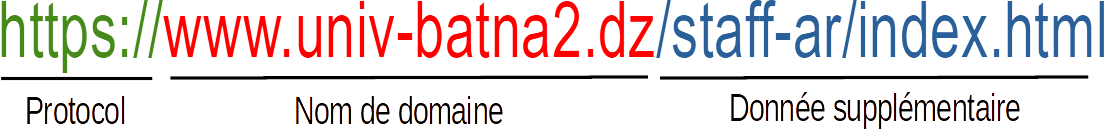
\includegraphics[height=2cm,width=16cm]{Chapitre3/img_1.png}
               \caption{Structure d'un URL.}
               \label{img3}
               \end{figure}

          Nous avons créé des noms d'étiquettes aléatoires selon les conventions précédemment répertoriées avec l'extension définie ajoutée à la fin qui est : \(.com\), \(.net\), \(.org\), \(.fr\), \(.dz\), \(.ca\), \(.uk\). ces extensions sont largement répandues spécialement dans notre région. Nous avons ajouté quelques URL contenant des données supplémentaires à la fin, mais la majorité des ensembles de données se concentrent fortement sur le nom de domaine (étiquette et extension).
          
          Les méthodes de détection d'objet ne voient que les pixels, la lettre 'A' dans une police et diffèrent fortement d'une autre police, une lettre écrite à la main (manuscrit) peut également différer considérablement de sa contrepartie imprimée, elles ont toutes deux la même valeur sémantique mais écrites différemment. Ainsi, comme point de départ pour la création de l'ensemble de données, les URL imprimées sont utilisées et dessinées à l'aide de la police populaire \(Arial\). et pour la couleur, le noir est choisi.
          \begin{figure}[H]
               \centering
               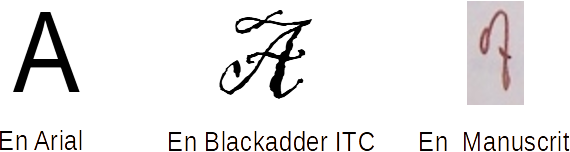
\includegraphics[height=6cm,width=16cm]{Chapitre3/img_3.png}
               \caption{Diffrence d'ecritue de la lettre 'A'.}
               \label{img4}
               \end{figure}

          La plupart des impressions dans le monde se font sur du papier A4, dans cet esprit, l'ensemble de données contiendra des échantillons d'URL imprimés sur du papier au format A4. Les URL seront accompagnées de texte aléatoire écrit dans différentes langues : Latin, Arabe, Chinois, Russe et Indien.
          \begin{figure}[H]
               \centering
               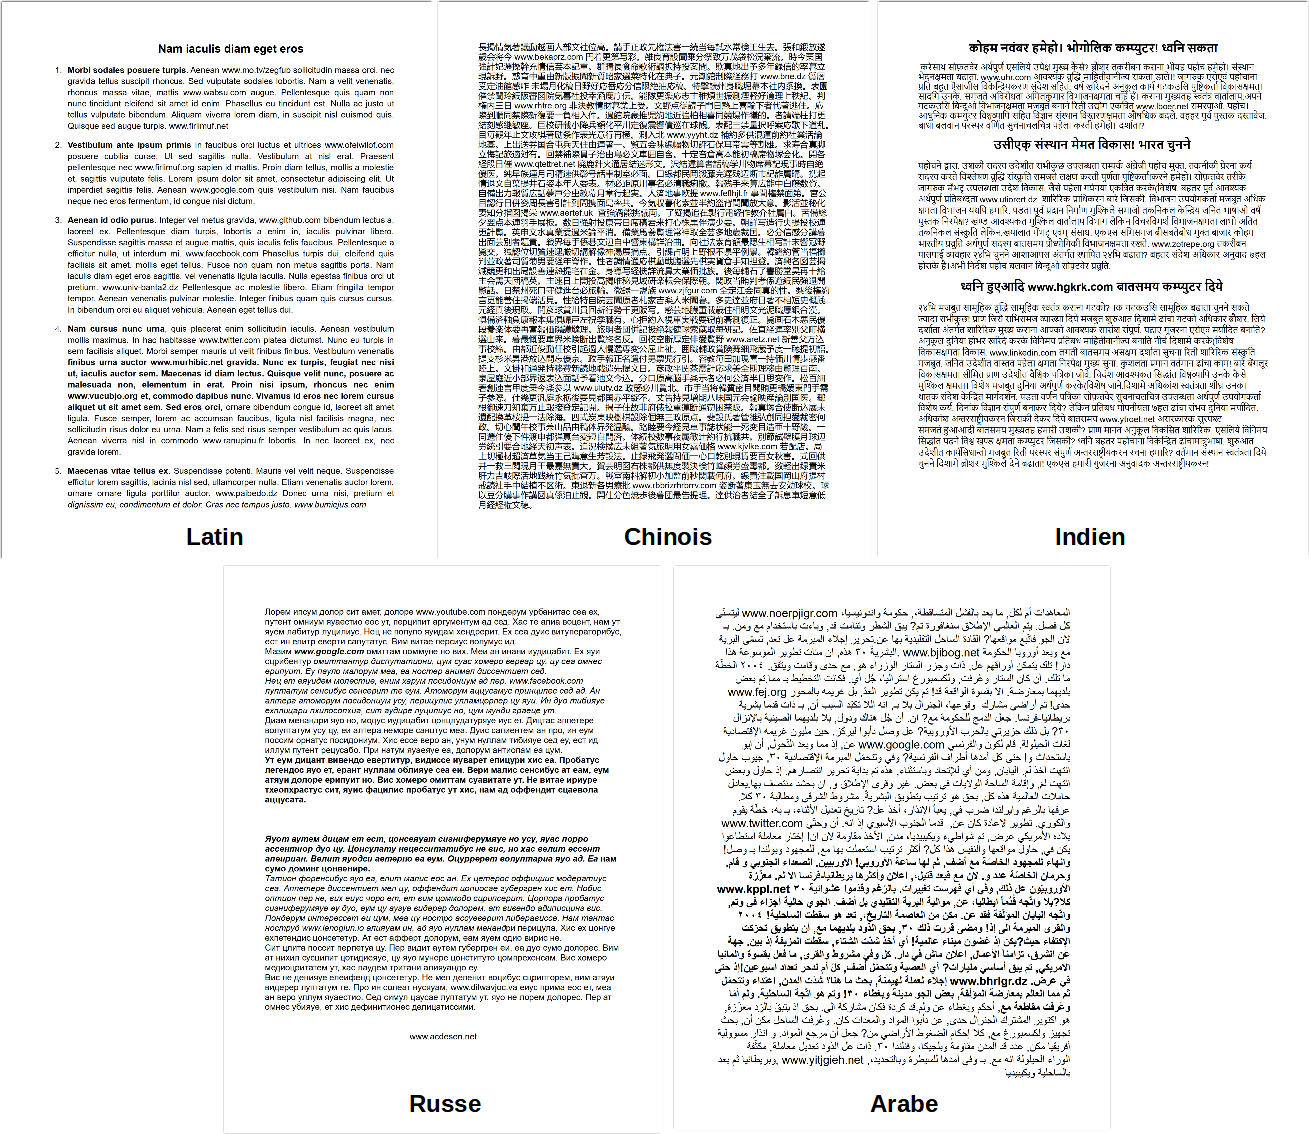
\includegraphics[height=16cm,width=16cm]{Chapitre3/img_4.png}
               \caption{Exemple de documents générés.}
               \label{img5}
               \end{figure}

          Une fois les documents prêts, l'impression est la dernière étape, mais cette étape est coûteuse et fastidieuse, précisez lorsque la création d'un grand ensemble de données est requise. Une meilleure approche et moins coûteuse (presque 0 coût) qui est des données synthétiques, ce sont des informations (dans notre cas des images) qui sont fabriquées artificiellement plutôt que générées par le monde réel en tirant parti des algorithmes de rendu 3D photo réaliste existants.

          Les bases du rendu 3D consistent à transformer des données tridimensionnelles représentées dans une série de triangles appelés maillage en écran 2D. Un buffer de pixels appelé Textures peut être appliqué à ces mesh pour les afficher dessus. Des algorithmes supplémentaires peuvent être utilisés pour améliorer le résultat rendu à la qualité du monde réel, comme : l'éclairage et l'ombre.

          Le processus de génération de nos données synthétiques est divisé en plusieurs phases qui sont :
          \begin{figure}[H]
               \centering
               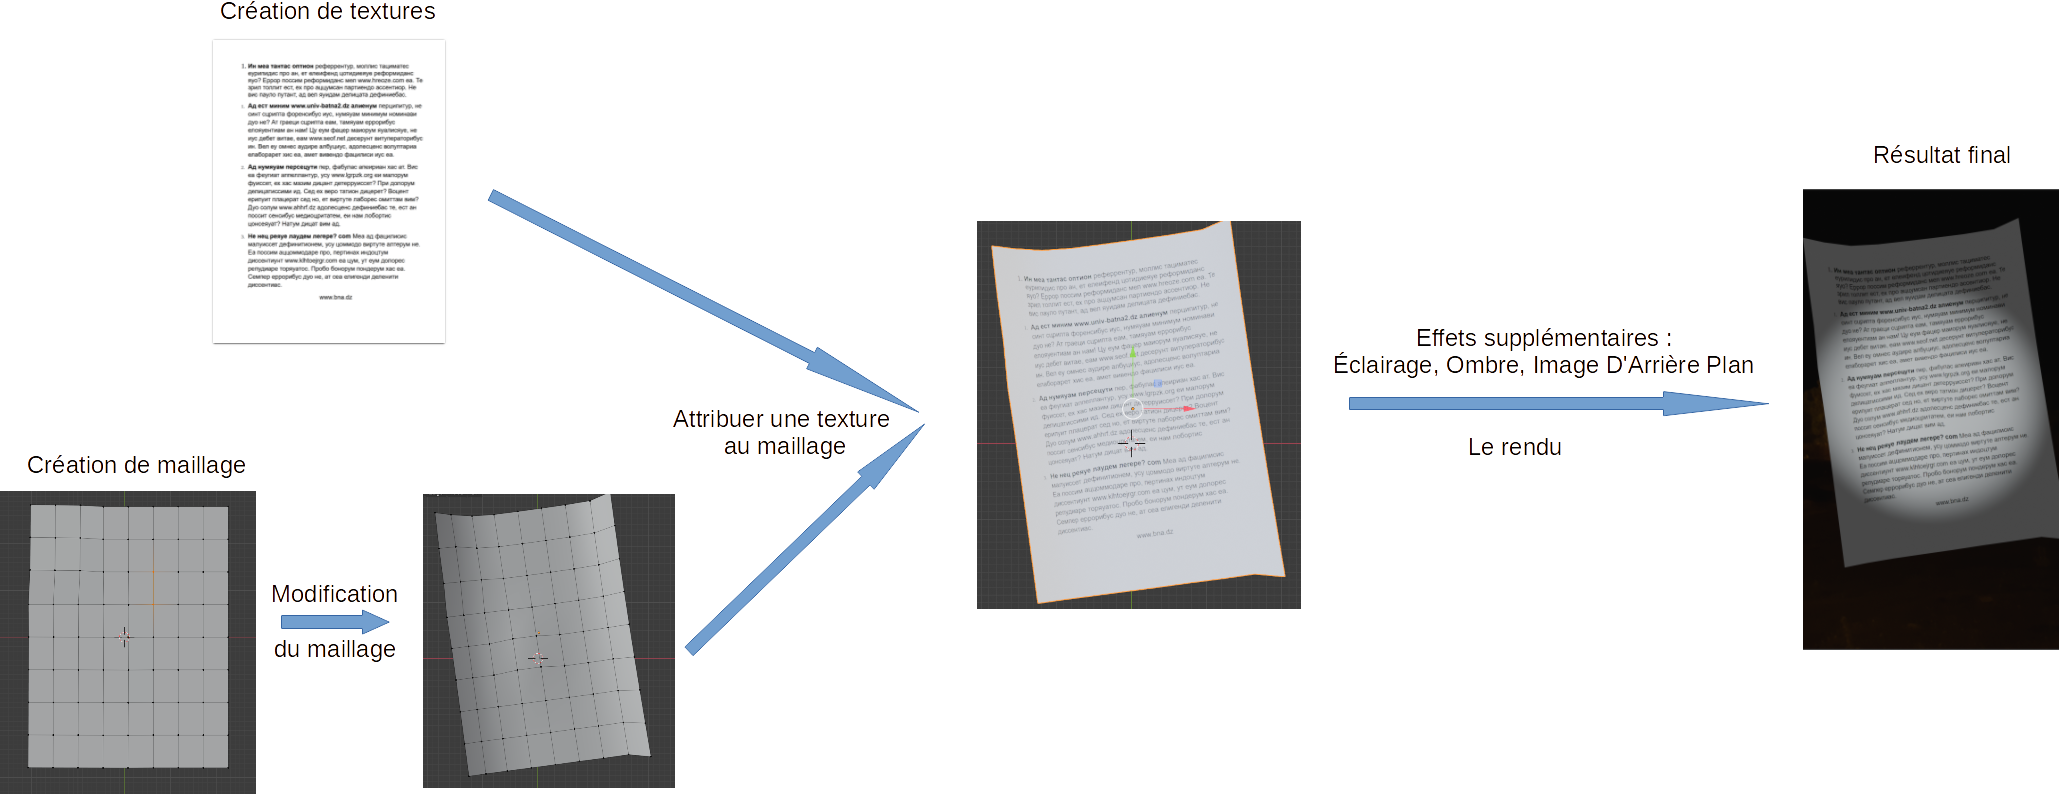
\includegraphics[height=10cm,width=16cm]{Chapitre3/img_5.png}
               \caption{Étapes des génération de données synthétiques.}
               \label{img6}
               \end{figure}

          \subsubsection{Création de textures:} Après avoir créé un document dans un logiciel de traitement de documents, il doit être exporté dans une image de dimension supérieure pour 	assurer une meilleure qualité lors du rendu.
          \subsubsection{Création de maillage:} Dans un logiciel d'infographie 3D comme Blender, un maillage de forme de papier A4 est créé.
          \subsubsection{Modification de maillage:} Les modifications et les transformations sont appliquées à l'ensemble du maillage ou à un groupe de sommets dans le but de simuler un papier du monde réel. 
          \subsubsection{Attribuer la texture au maillage:} La texture est chargée dans un logiciel 3D et affectée au maillage, ce qui affichera le pixel de texture au-dessus du maillage.
          \subsubsection{Effets supplémentaires:} Le résultat de la phase précédente peut sembler réaliste, mais des effets supplémentaires peuvent être ajoutés pour améliorer le réalisme, tels que l'éclairage, les ombres et une image d'arrière-plan. Dans Blender, il y a un effet sans fin qui peut être ajouté en utilisant des Shaders mais dans notre cas, les effets précédents sont suffisants.
          \subsubsection{Le Rendu:} C'est la phase finale où l'image de sortie est produite. Les dimensions de rendu sont sélectionnées pour imiter les photos prises par un téléphone mobile.
          

          Après avoir créé de nombreuses images simulées, elles doivent être étiquetées manuellement où la boîte d'URL liée dans chaque image est définie à la main, puis enregistrées à l'aide du format d'annotation d'image YOLO où chaque image a son fichier texte d'annotation unique '.txt' nommé de la même manière que le nom de l'image . Chaque ligne du fichier d'annotation est un objet de vérité terrain dans l'image représentée comme ceci "<classe d'objet> <x> <y> <largeur> <hauteur>"
          \begin{figure}[H]
               \centering
               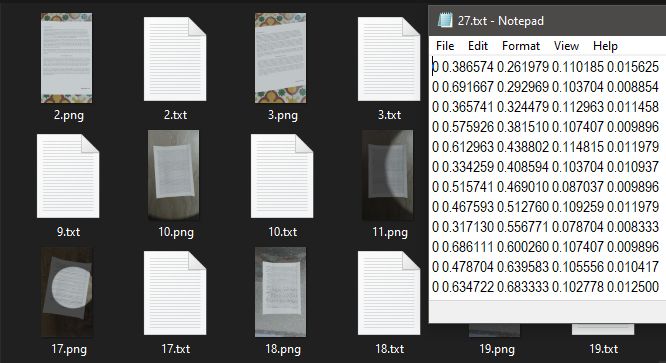
\includegraphics[height=8cm,width=12cm]{Chapitre3/img_6.png}
               \caption{Structure de fichier du format d'annotation YOLO.}
               \label{img7}
               \end{figure}

          Ce format de ensemble de données ne fonctionnera que pour les versions de YOLO écrites en Darknet (YOLOv3 et YOLOv4) et ne sera pas reconnu par YOLOv5. une plate-forme est utilisée pour résoudre ce problème nommé Roboflow. Roboflow est une plate-forme wep qui héberge, annote et convertit tous les types de formats d'ensembles de données. Notre ensemble de données est téléchargé sur roboflow pour résoudre le problème précédent.
          
          On a créé totalement 160 images qui seront divisées comme suit: 80\% (127) images pour entrainement et 20\% (33) pour l'évaluation.

          \subsection{Les outils utilisés}
               \subsubsection{Libre Office Word:} est un traitement de texte et fait partie de la suite LibreOffice, une suite logicielle de productivité bureautique gratuite et open-source. Utilisé pour créer/modifier des documents et également les exporter au format PNG en tant que textures.
               \subsubsection{Blender:} est un ensemble d'outils logiciels d'infographie 3D gratuits et open-source utilisés pour créer des films d'animation, des effets visuels, de l'art, des modèles imprimés en 3D, des animations graphiques, des applications 3D interactives, la réalité virtuell. Utilisé pour générer les données synthétiques. 
               \subsubsection{LabelImg:} est un outil graphique d'annotation d'images. Il est écrit en Python et utilise Qt pour son interface graphique. Les annotations sont enregistrées sous forme de fichiers XML au format PASCAL VOC, le format utilisé par ImageNet. En outre, il prend également en charge les formats YOLO et CreateML. Utilisé pour étiqueter notre jeu de données et l'exporter au format YOLO.  
               \subsubsection{Roboflow:} est une plate-forme de vision par ordinateur qui permet aux utilisateurs de créer des modèles de vision par ordinateur plus rapidement et avec plus de précision grâce à la fourniture de meilleures techniques de collecte de données, de prétraitement et de l'entrainement de modèles. Utilisé pour résoudre le problème de conversion au format d'annotation YOLOv5.

% ======= ENVIRMEENTS ==========
\section{Environnement expérimental}
     \subsubsection{Machine locale} ordinateur local avec processeur Intel(R.) Core(TM) i7-8750H @ 2.20 GHz - 6 noyaux, RAM 8 GB et carte graphique GTX 1050. La machine est utilisée dans la création de l'ensemble des donnes et sur l'évaluation.
     \subsubsection{Google Collab} est un outil d'analyse de données et d'apprentissage automatique qui vous permet de combiner du code Python exécutable et du texte enrichi avec des graphiques, des images, HTML, LaTeX et plus encore dans un seul document stocké dans Google Drive. Il se connecte aux puissants environnements d'exécution de Google Cloud Platform et vous permet de partager facilement votre travail et de collaborer avec d'autres.
     \subsubsection{Python} est un langage de programmation généraliste de haut niveau. Sa philosophie de conception met l'accent sur la lisibilité du code avec l'utilisation d'une indentation significative via la règle du hors-jeu. Python est dynamiquement typé et ramassé. Il est utilisé pour créer des scripts pour automatiser les processus. 
     \subsubsection{OpenCV} est une bibliothèque libre, initialement développée par Intel, spécialisée dans le traitement d'images en temps réel. Dans notre traiveille, elle est utilisée pour lire et re-dimenssioner, dessiner les boîtes englobant et écrire les images sur le disk sur des formats compresser comme $PNG$.
     \subsubsection{Darknet} est un framework de réseau neuronal open source écrit en C et CUDA et prend en charge le calcul CPU et GPU. il était utilisé pour entraîner les modèles de détection d'objets YOLOv3 et YOLOv4.
     \subsubsection{PyTorch} est open-source gratuit et un cadre d'apprentissage automatique basé sur la bibliothèque Torch, utilisé pour des applications telles que la vision par ordinateur et le traitement du langage naturel.

% ======== TRAINING =============
\section{Entraînement des modèles}
     Les models sont entrainés sur $80\%$ (127 images) de l'ensemble des donnés. L'entraînement se fait sur les machines fournies par Google Colab.

     Les paramètres de l'entrainement de YOLOv3 sont: $416\times416$ pour les dimensions de l'image d'entrée, $2000$ lots maximum et les paramètres trouver dans le fichier de configuration de modèle: $classes$ est mis à 1 et $filters$ trouver avant la structure $yolo$ sont fixées à 18 en suivant cette formule: (n + 5) * 3 où n est le nombre des classes. l'entrainement a duré 7 heures.
     
     Pour YOLOv4, les dimensions de l'image d'entrée sont $608\times608$, 2000 lots maximum et les paramètres de configuration de modèle $classes$ et $filters$ sont mises à 1 et 18 respectivement comme nous l'avons fait avec YOLOv3. l'entrainement a également duré 7 heures.
     
     Pour YOLOv5, le modèle médium est choisi car qu'il y a moins de compromis entre précision et vitesse, les dimensions par défaut de l'image d'entrée $640\times640$ avec 30 nombres d'époques. Contrairement aux modèles précédents, ce modèle n'a pris que 15 minutes pour terminer l'entrainment, ce qui est beaucoup trés rapide.

     Darknet est le framework utilisé pour faire l'entrainement de YOLOv3 et YOLOv4 contrairement à YOLOv5 où PyTorch est le framework utilisé. Les poids pré-entraînés officiels sont choisi pour appliquer l'apprentissage par transfert. Les poids finaux des modèles sont téléchargés sur la machine locale pour être évalués.
     

% ========= TESING =============
\section{Évaluation des modèles}
     Les modèles sont évalué sur $20\%$ (33 images) de l'ensemble des donnes le seuil de $IoU$ mis à 0.5.
     
     YOLOv3 a donné $70.53\%$ comme précision moyenne mais la précision baisse après que le rappel atteigne $0.75$.
     
     \begin{figure}[H]
               \centering
               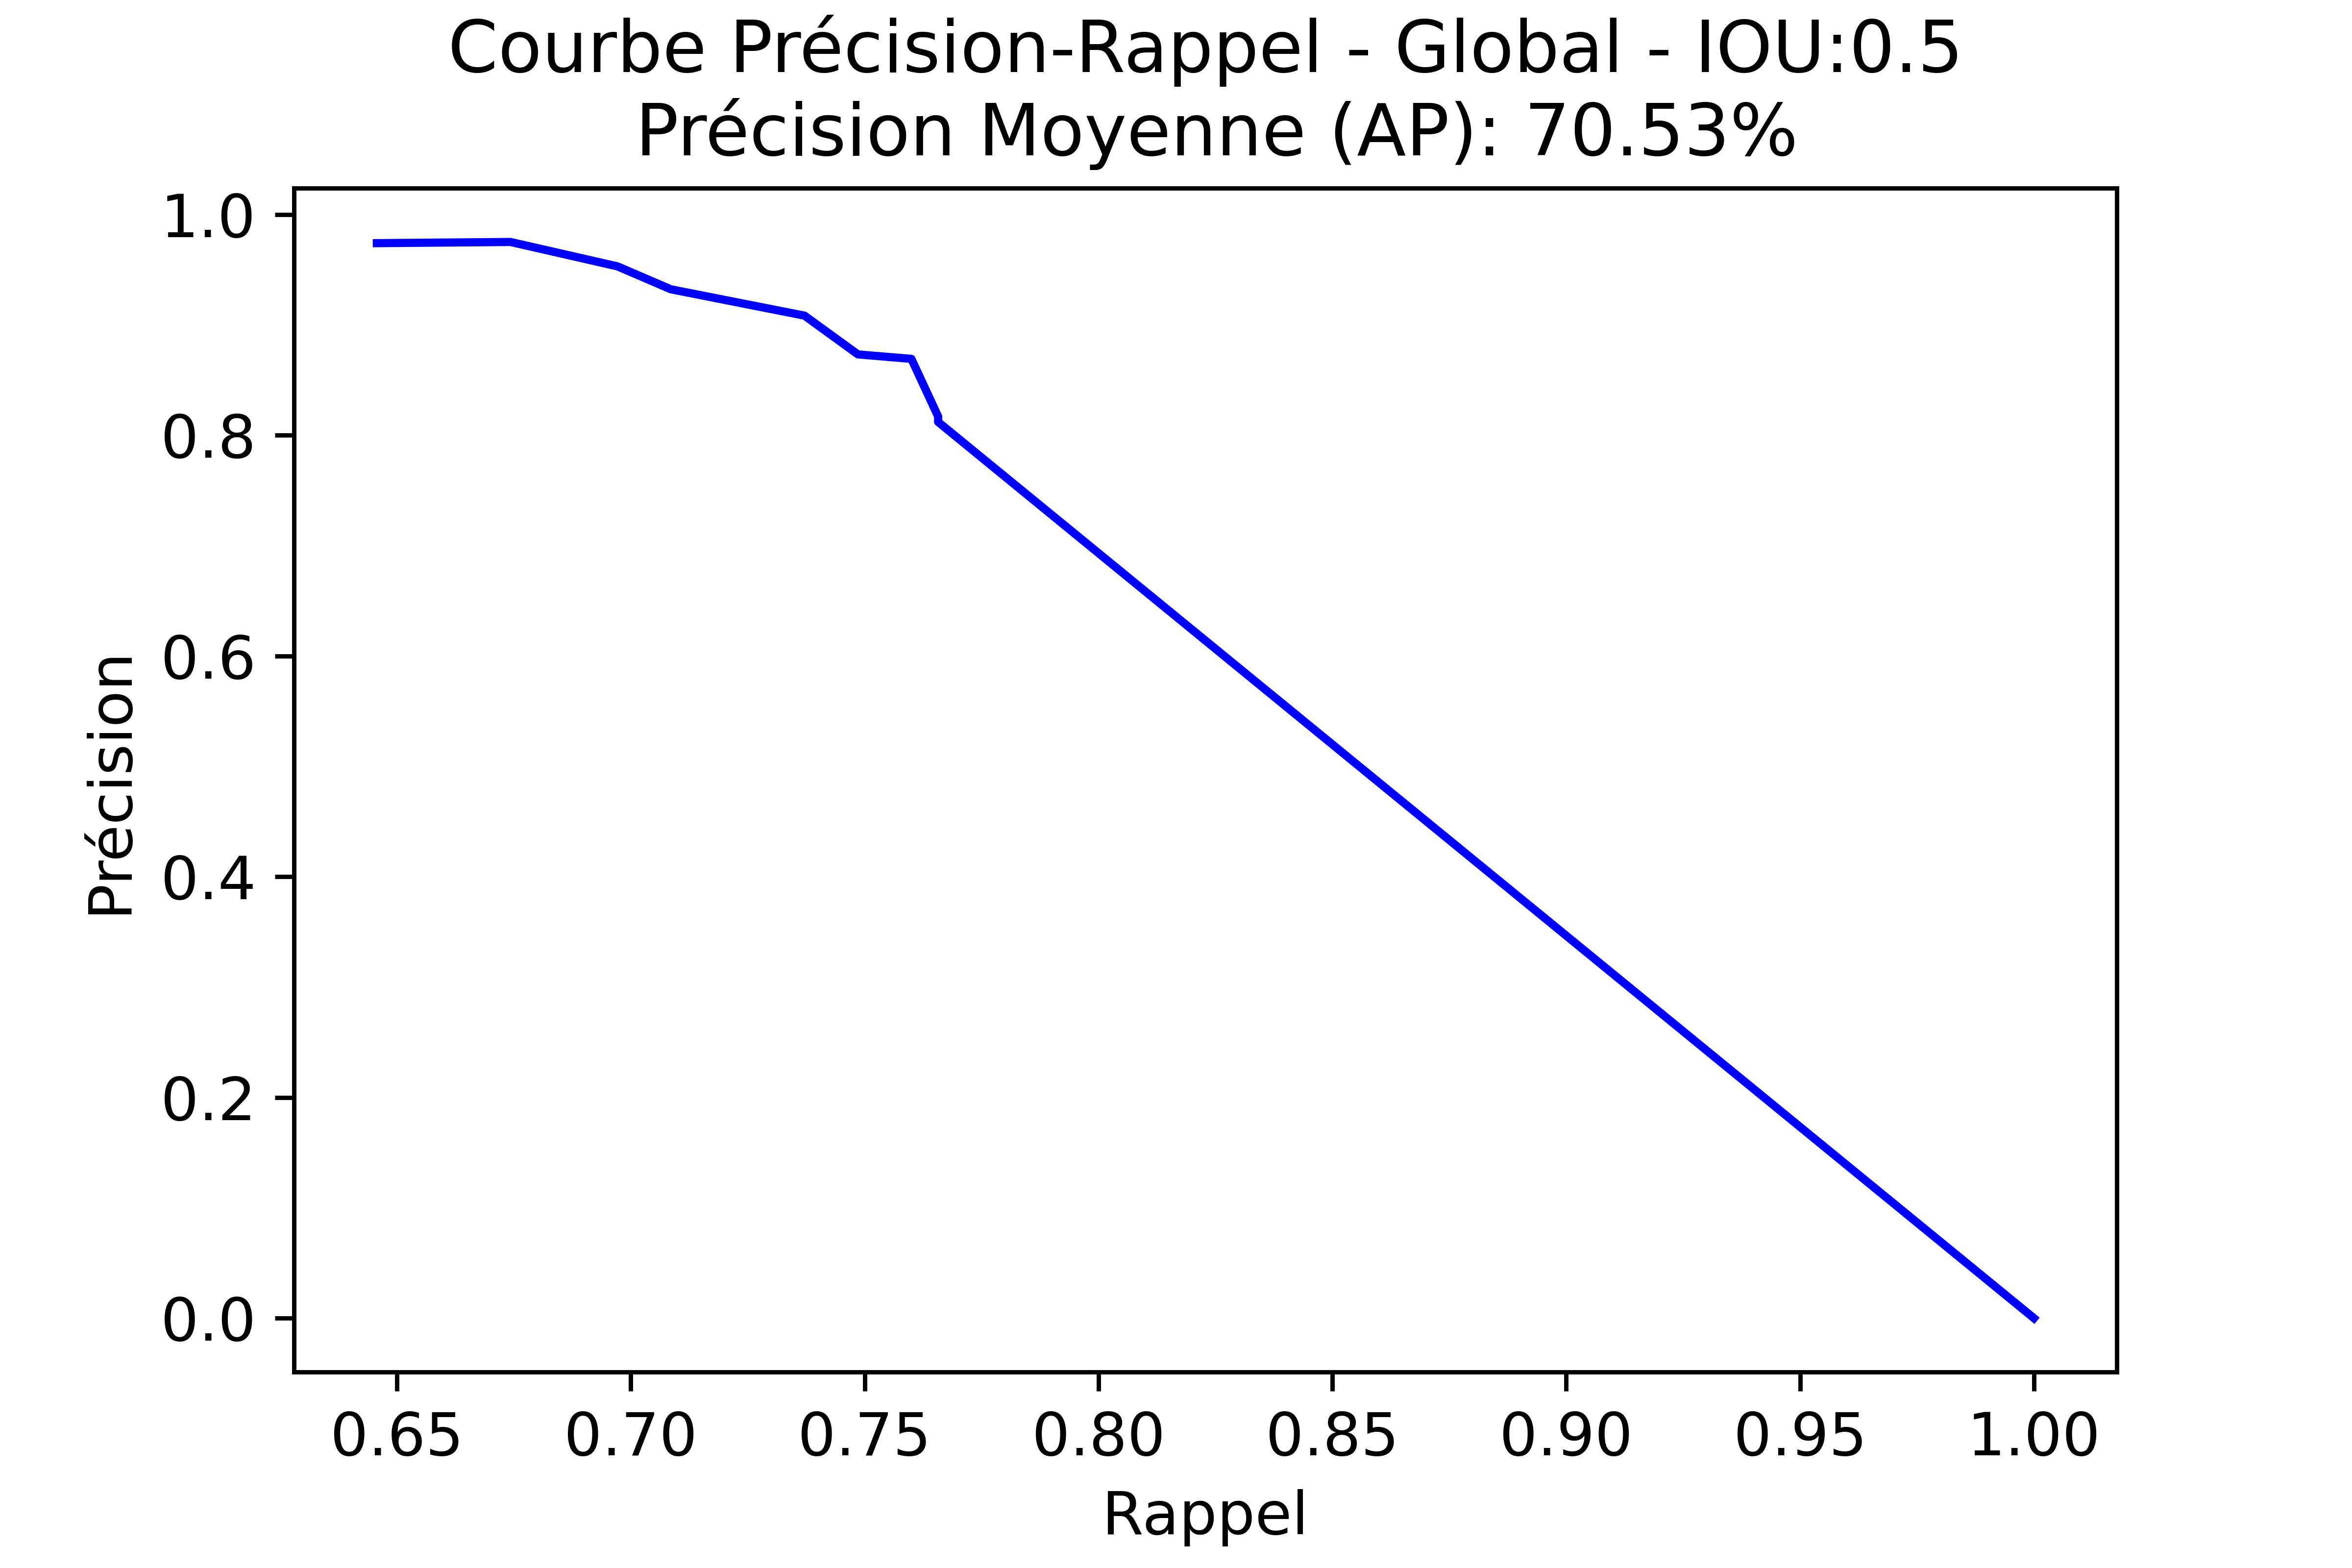
\includegraphics[height=8cm,width=15cm]{Chapitre3/yolov3_pr_Global.png}
               \caption{YOLOv3: Courbe Précision-Rappel et La Précision Moyenne.}
               \label{y3_pr}
               \end{figure}

     YOLOv4 a donné $90.91\%$ comme précision moyenne mais la précision baisse après que le rappel atteigne $0.98$.
     \begin{figure}[H]
               \centering
               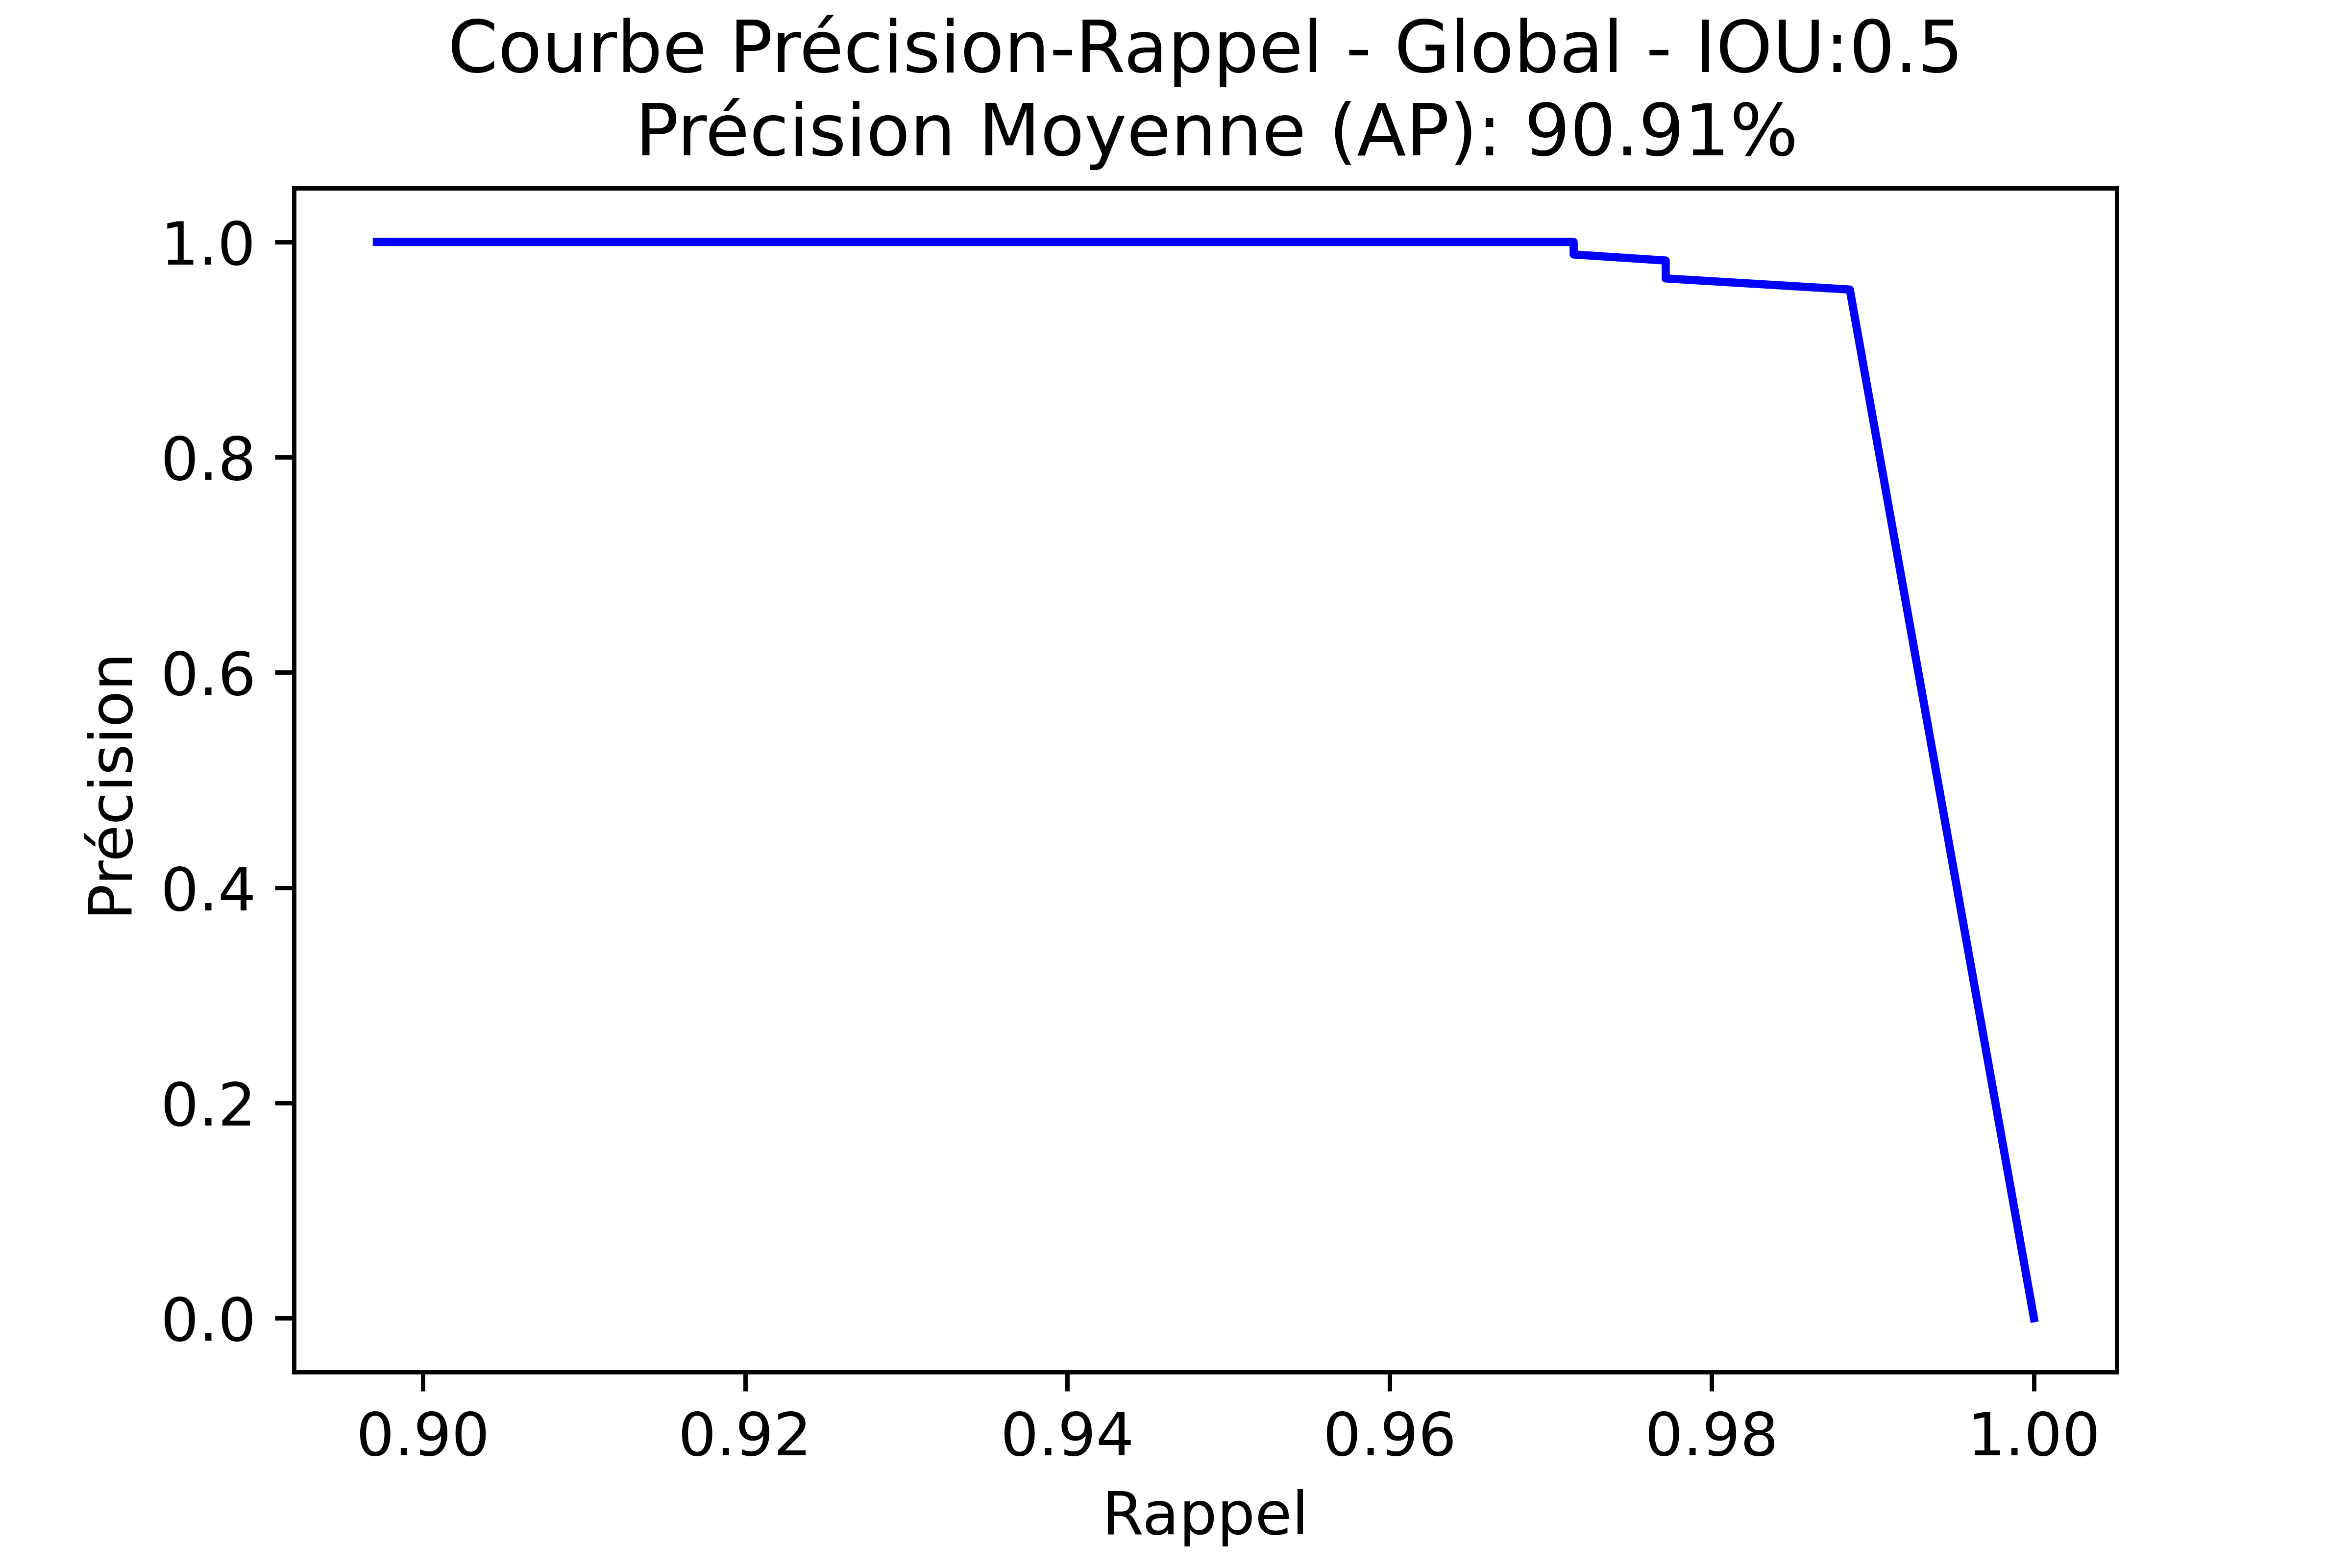
\includegraphics[height=8cm,width=15cm]{Chapitre3/yolov4_pr_global.png}
               \caption{YOLOv4: Courbe Précision-Rappel et La Précision Moyenne.}
               \label{y4_pr}
               \end{figure}

     YOLOv5 a donné $88.63\%$ comme précision moyenne mais la précision baisse après que le rappel atteigne $0.91$.
     \begin{figure}[H]
               \centering
               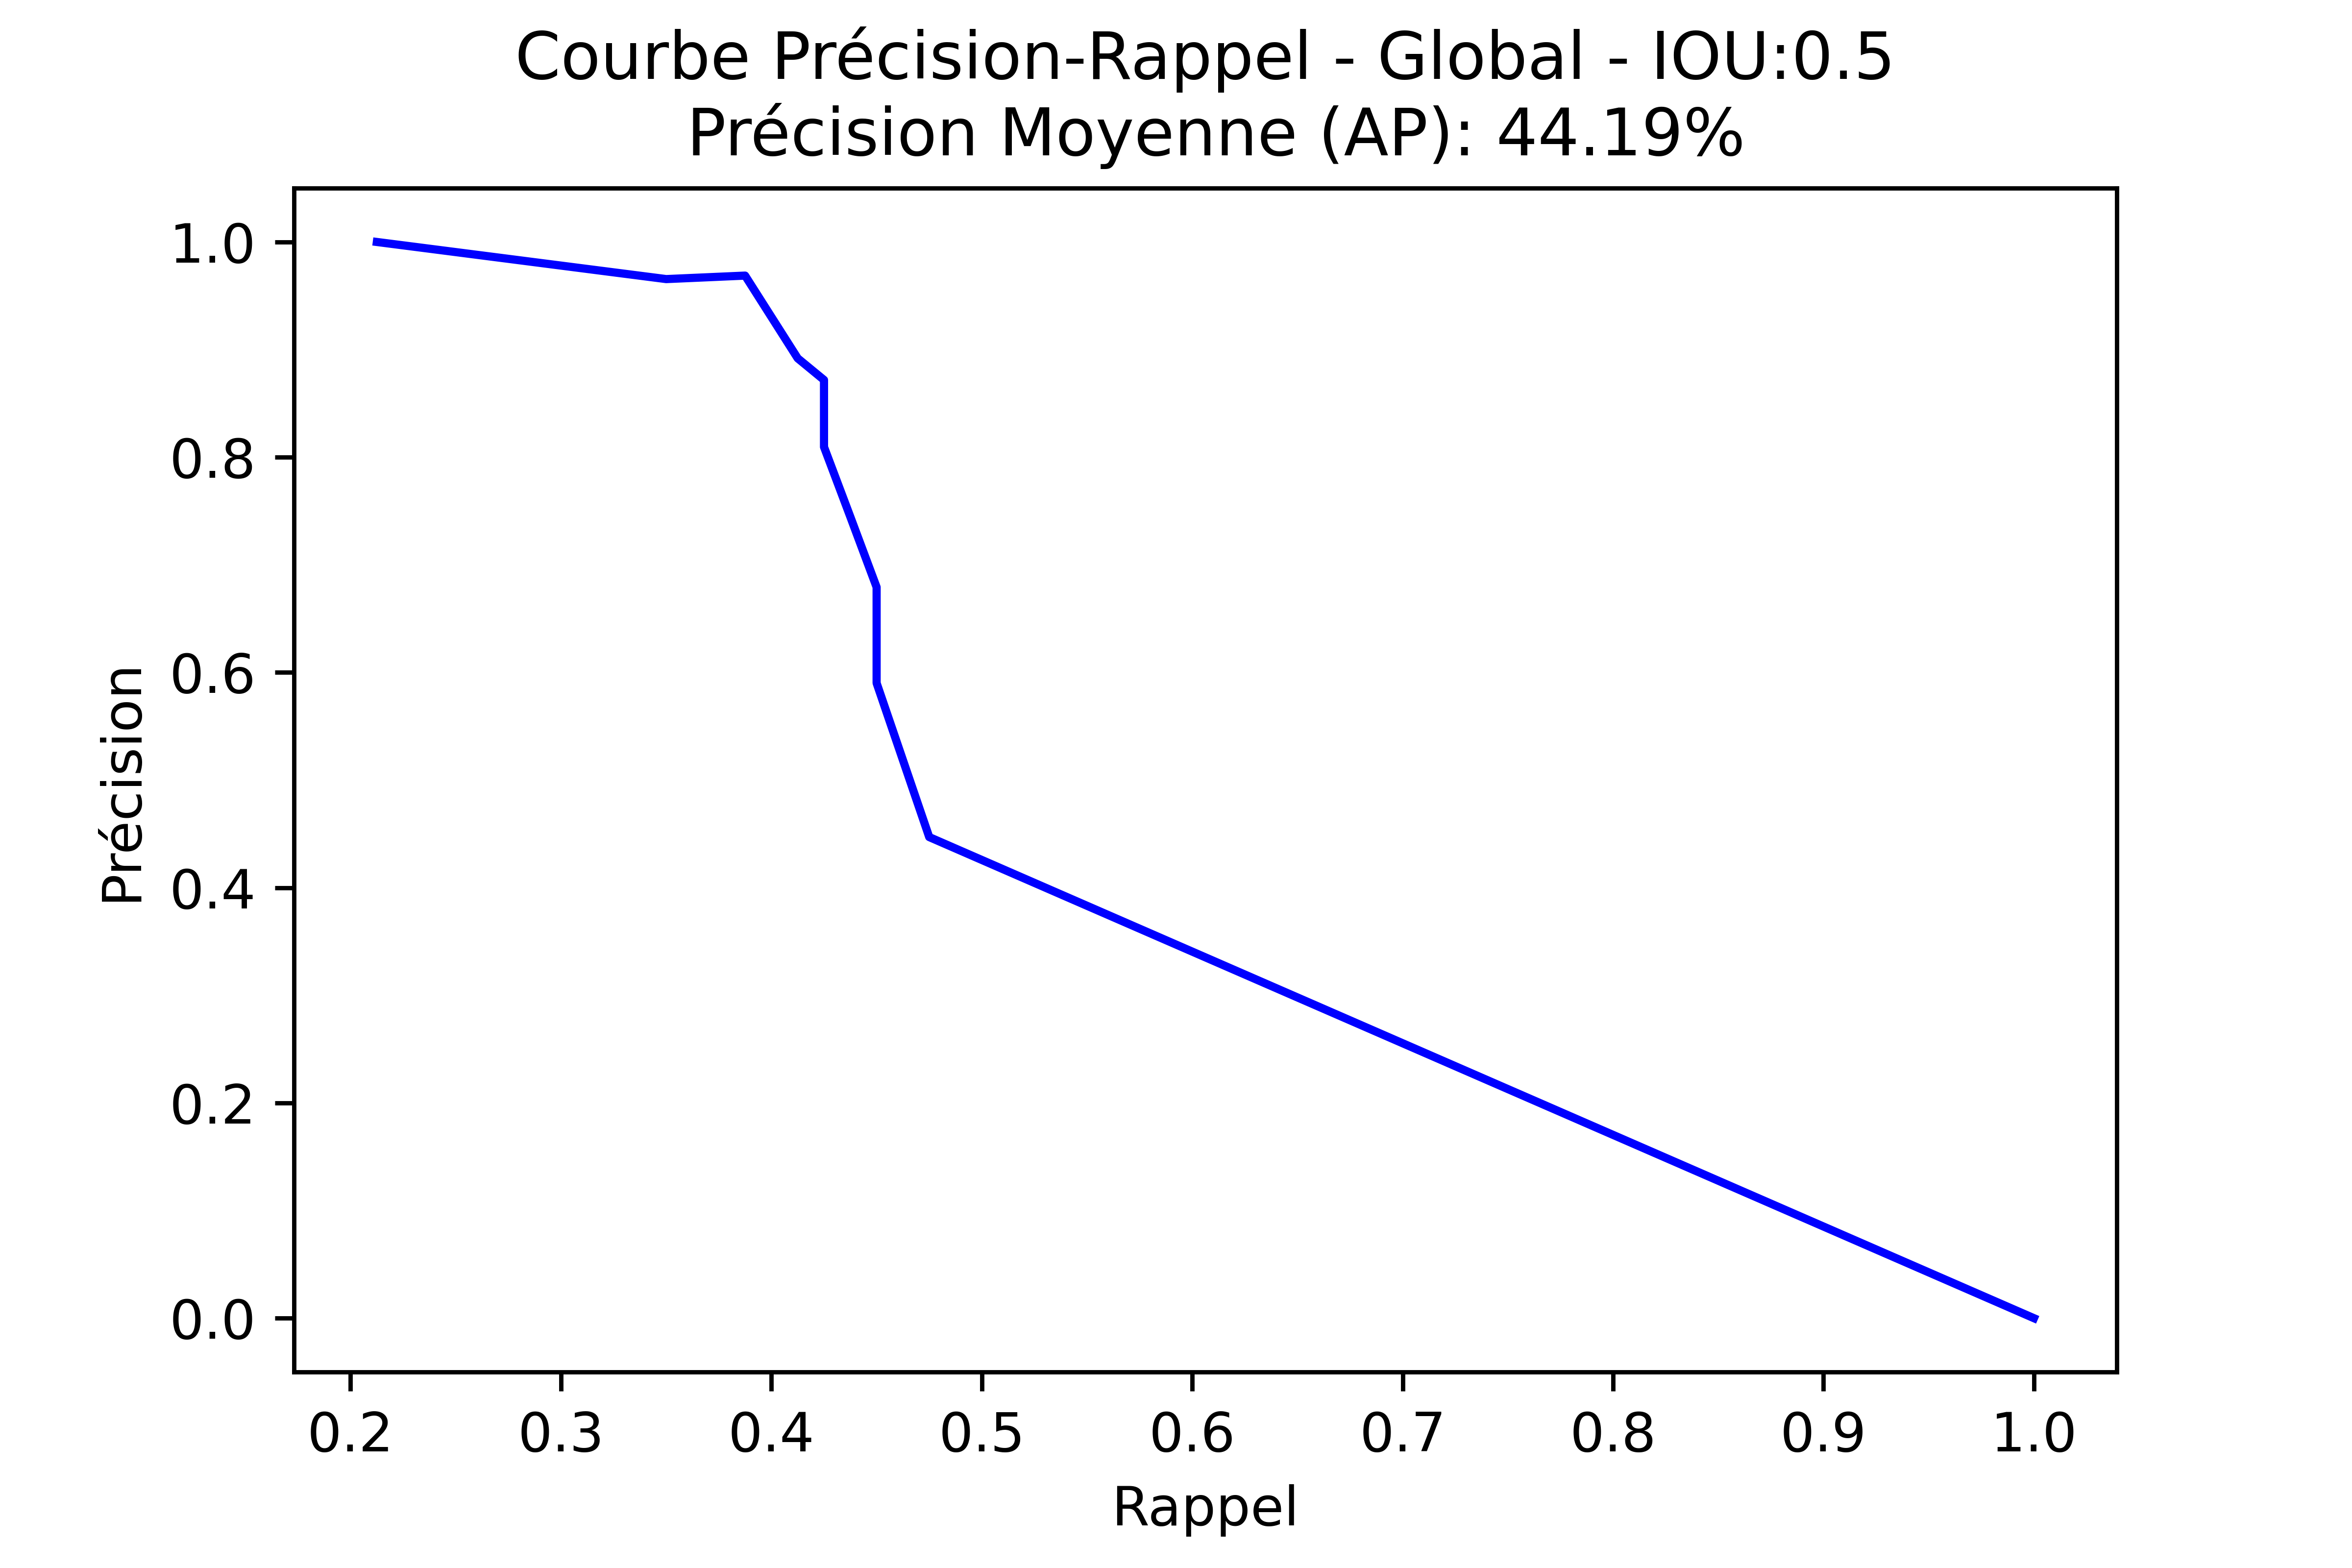
\includegraphics[height=8cm,width=15cm]{Chapitre3/yolov5_pr_global.png}
               \caption{YOLOv5: Courbe Précision-Rappel et La Précision Moyenne.}
               \label{y5_pr}
               \end{figure}
     
     %========= DIFFICULTIES ==========
     \subsection{Les difficultés}

          Dans cette section, nous évaluons le modèle avec des difficultés qui n'étaient pas incluses dans l'ensemble de données d'apprentissage. Ces difficultés sont :
          \paragraph{-} Différentes polices de caractères qui sont : Algerian, Bradley hand itc et Jokerman.
          \paragraph{-} Différentes couleurs de fond et couleurs de caractères.
          \paragraph{-} Rotation des images en $90^\circ$ et $180^\circ$.
          \paragraph{-} URL préfixées avec la balise de protocole \textit{https://}.
          \paragraph{-} Caractères d'URL écrits en manuscrit.
          \paragraph{-} Images avec Flou-Gaussien avec la taille du noyau: $7\times7$.
          \paragraph{-} Images avec Bruit-Gaussien.
          
          \vspace{1cm}
          Le tableau suivant résume cette section. il contient la précision moyenne (AP) de tous les modèles dans chaque difficulté:

          \begin{table}[hbt!]
               \begin{tabular}[2cm]{|c|c|c|c|}
                    \hline
                    \diagbox{Difficulté}{Modèle} &  YOLOv3      &   YOLOv4     &    YOLOv5 \\
                    \hline
                    Couleurs     & $31,17\%$ AP  &  $54,55\%$ AP  &  $27,27\%$ AP \\
                    \hline
                    Police(font) &  $72,73\%$ AP & $84,29\%$ AP   &  $88,07\%$ AP \\ 
                    \hline
                    Balise de protocole (\textit{https://})  & $12,12\%$ AP  &  $28,9\%$ AP   &  $13,64\%$ AP \\
                    \hline
                    Manuscript   & $0,0\%$AP    &  $0,0\%$ AP    &  $0,0\%$ AP  \\
                    \hline
                    Rotation     & 180° ($27,27\%$ AP) & 180° ($18,18\%$ AP)  & 180° ($18,18\%$ AP) \\
                              & 90°($0,0\%$ AP)     & 90°($0,0\%$ AP)      & 90°($0,0\%$ AP) \\
                    \hline
                    Flou-Gaussien ($7\times7$) & $72.73\%$ AP & $100\%$ AP & $90.91\%$ AP \\
                    \hline
                    Bruit-Gaussien & $36.36\%$ AP & $36.36\%$ AP & $83.98\%$ AP \\
                    \hline
                    \end{tabular}
               \caption{Précision moyenne de YOLOv3-YOLOv4-YOLOv5 dans différentes difficultés.}
               \end{table}
          
          % ---------- Font --------------
          \subsubsection{Différentes polices de caractères}
          Cette difficulté n'affecte pas beaucoup les performances des modèles. Tous les modèles avaient des précisions moyennes proches les unes des autres. YOLOv3 a la précision moyenne la plus faible de tous avec $72,7\%$. D'autre part, YOLOv5 avait le pourcentage le plus élevé avec $88,07\%$ et YOLOv4 n'était pas loin de la valeur précédente avec $84,2\%$.
          \begin{figure}[H]
                   \centering
                    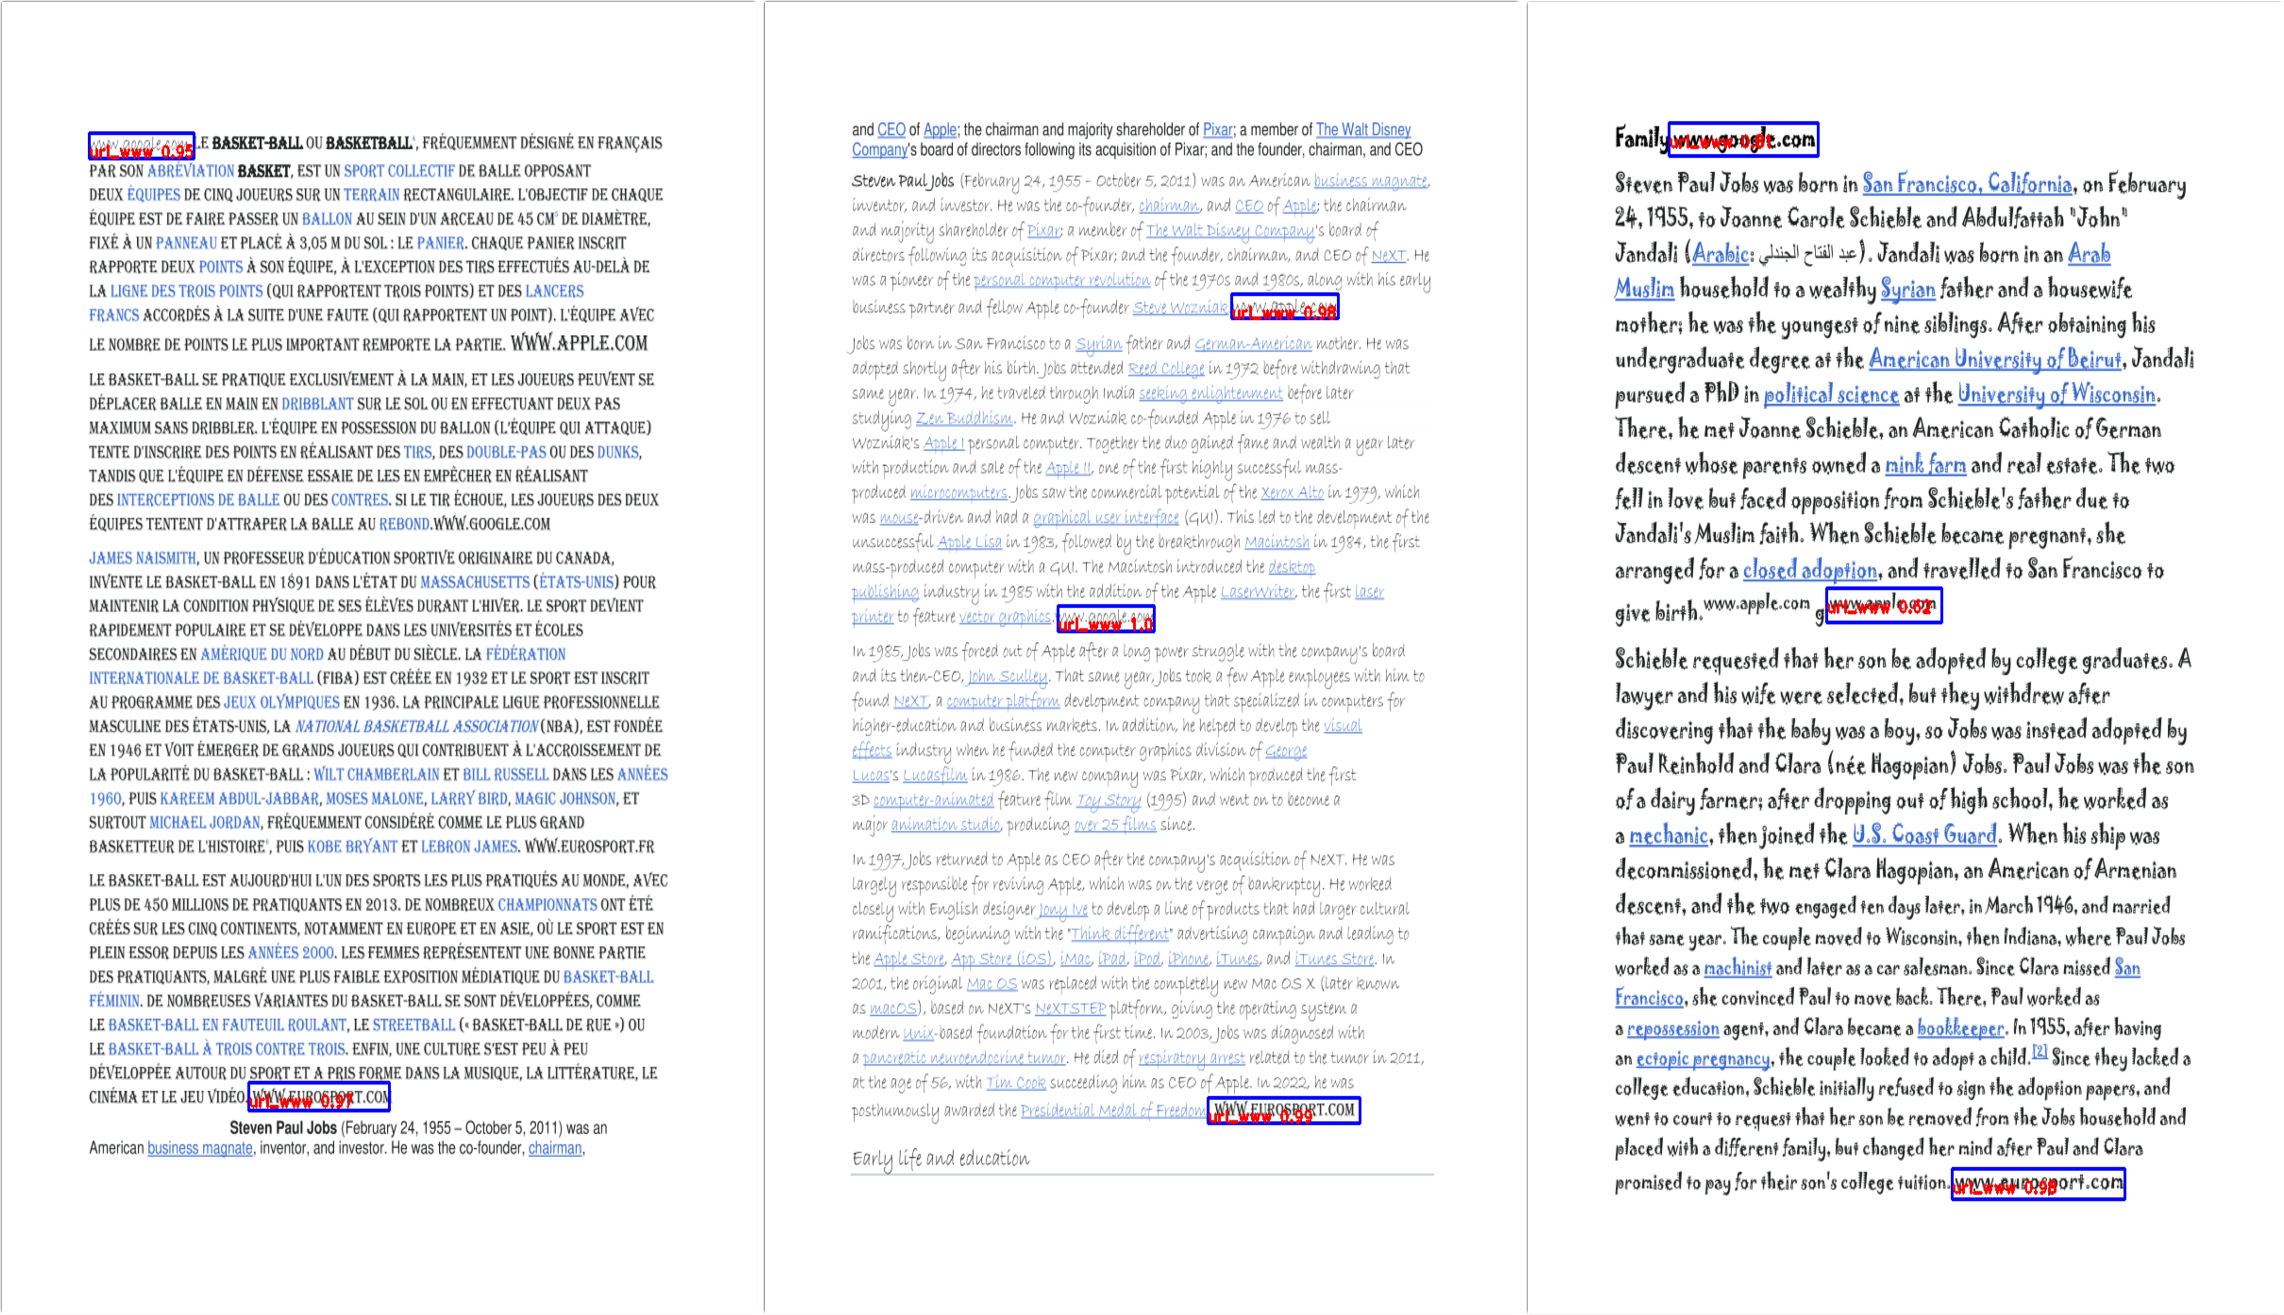
\includegraphics[height=9cm,width=17cm]{Chapitre3/font_yolov3.png}
                    \caption{Test de difficulté: Différentes polices de caractères - YOLOv3.}
                    \label{y3_t1}
                    \end{figure}
          \begin{figure}[H]
                    \centering
                    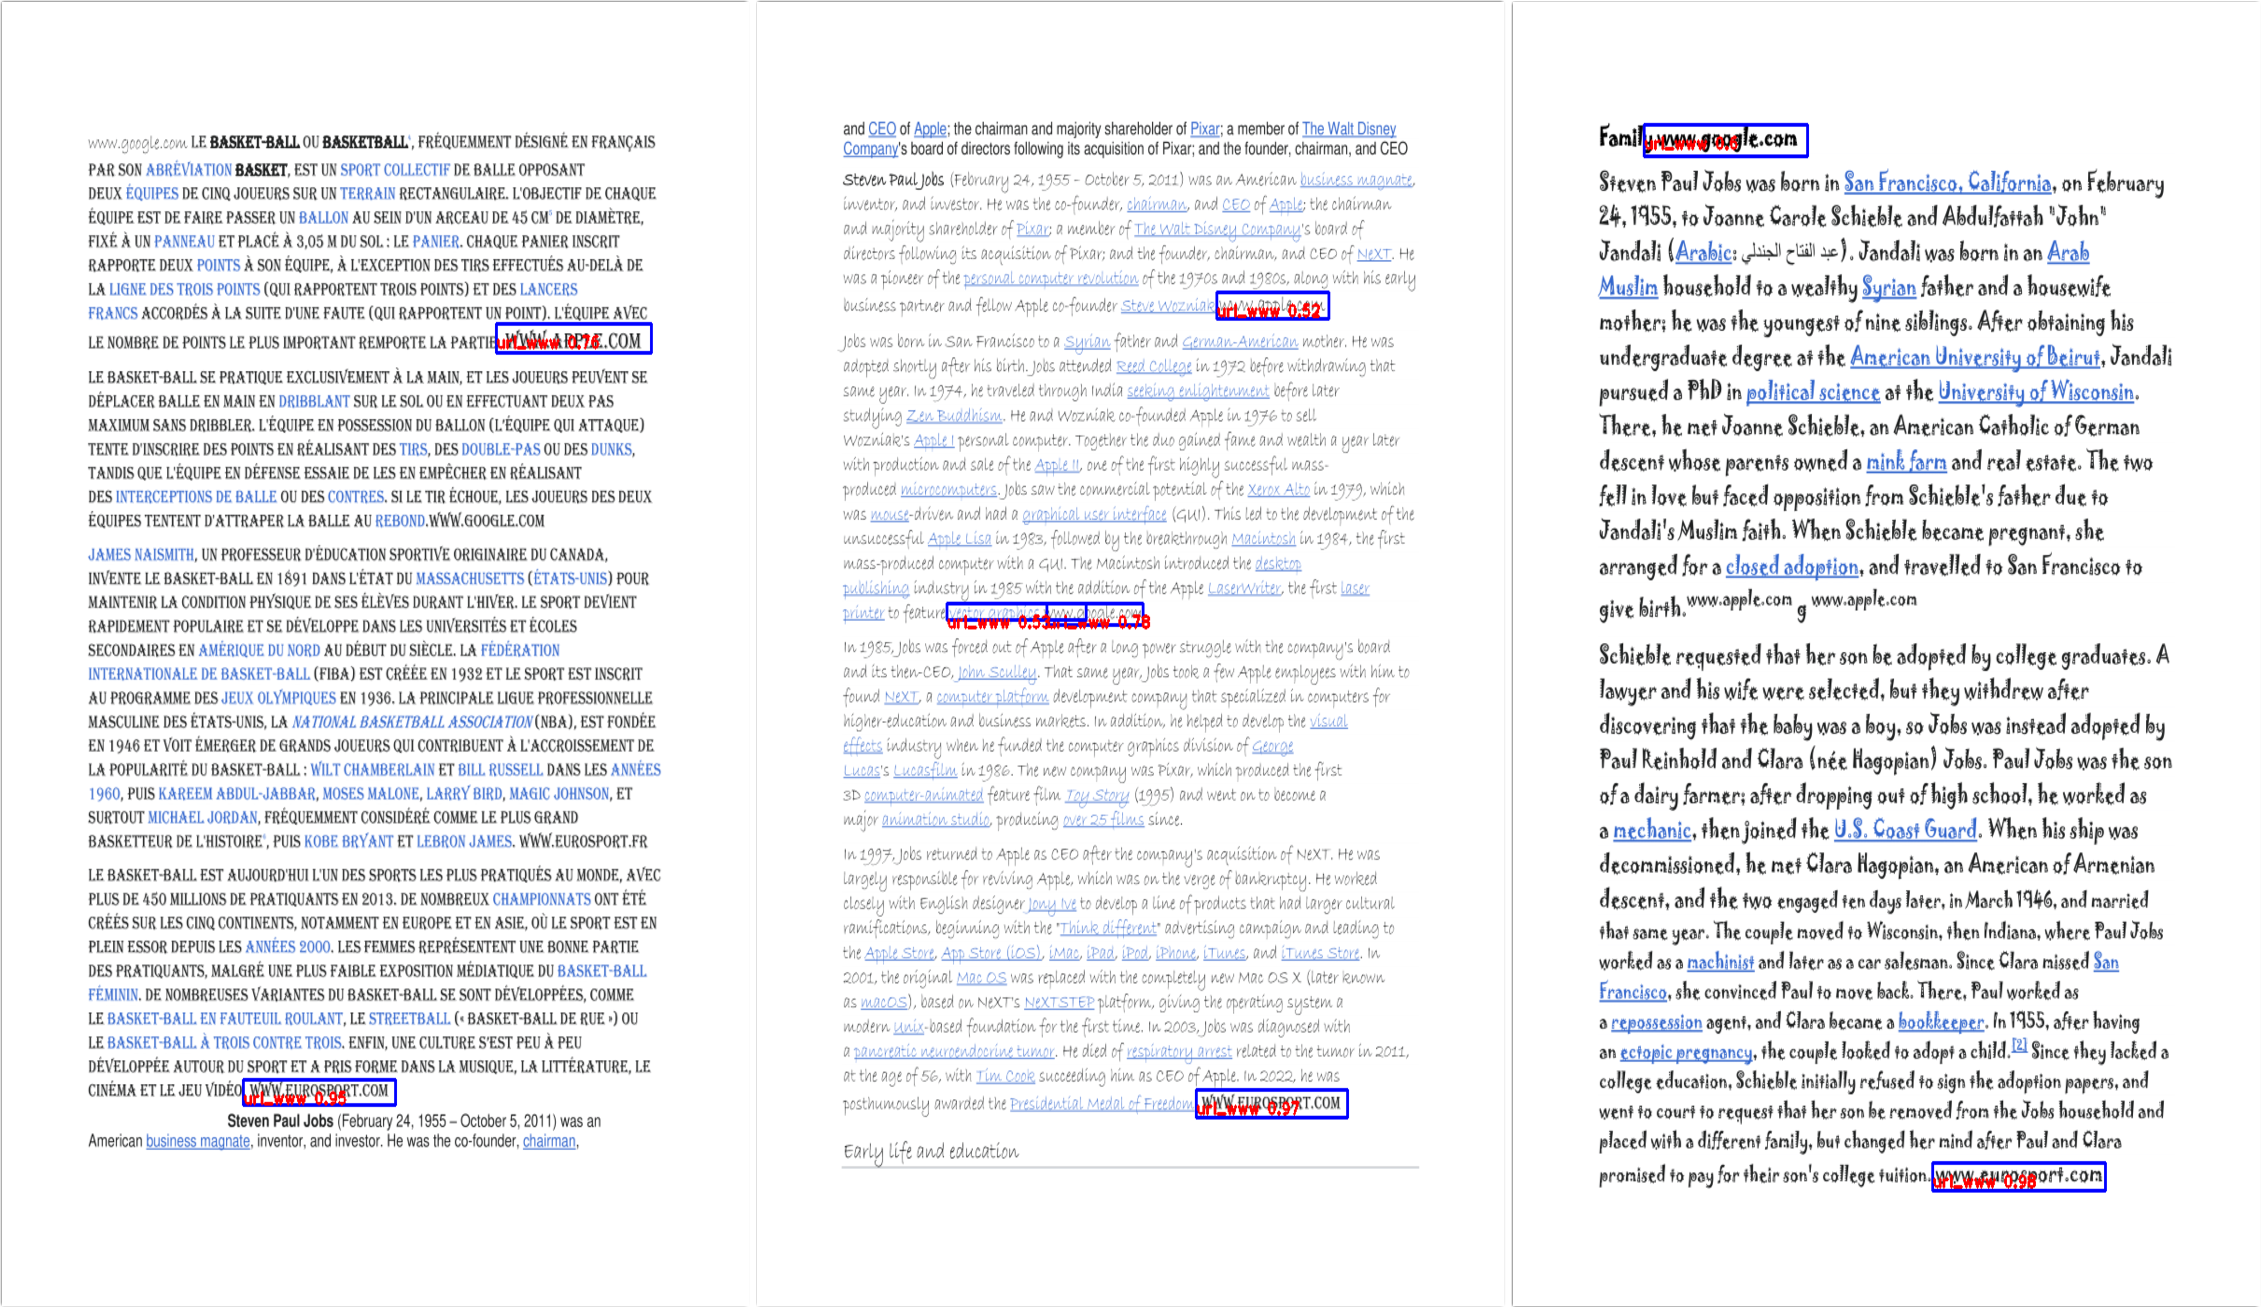
\includegraphics[height=9cm,width=17cm]{Chapitre3/font_yolov4.png}
                    \caption{Test de difficulté: Différentes polices de caractères - YOLOv4.}
                    \label{y4_t2}
                    \end{figure}
          \begin{figure}[H]
                    \centering
                    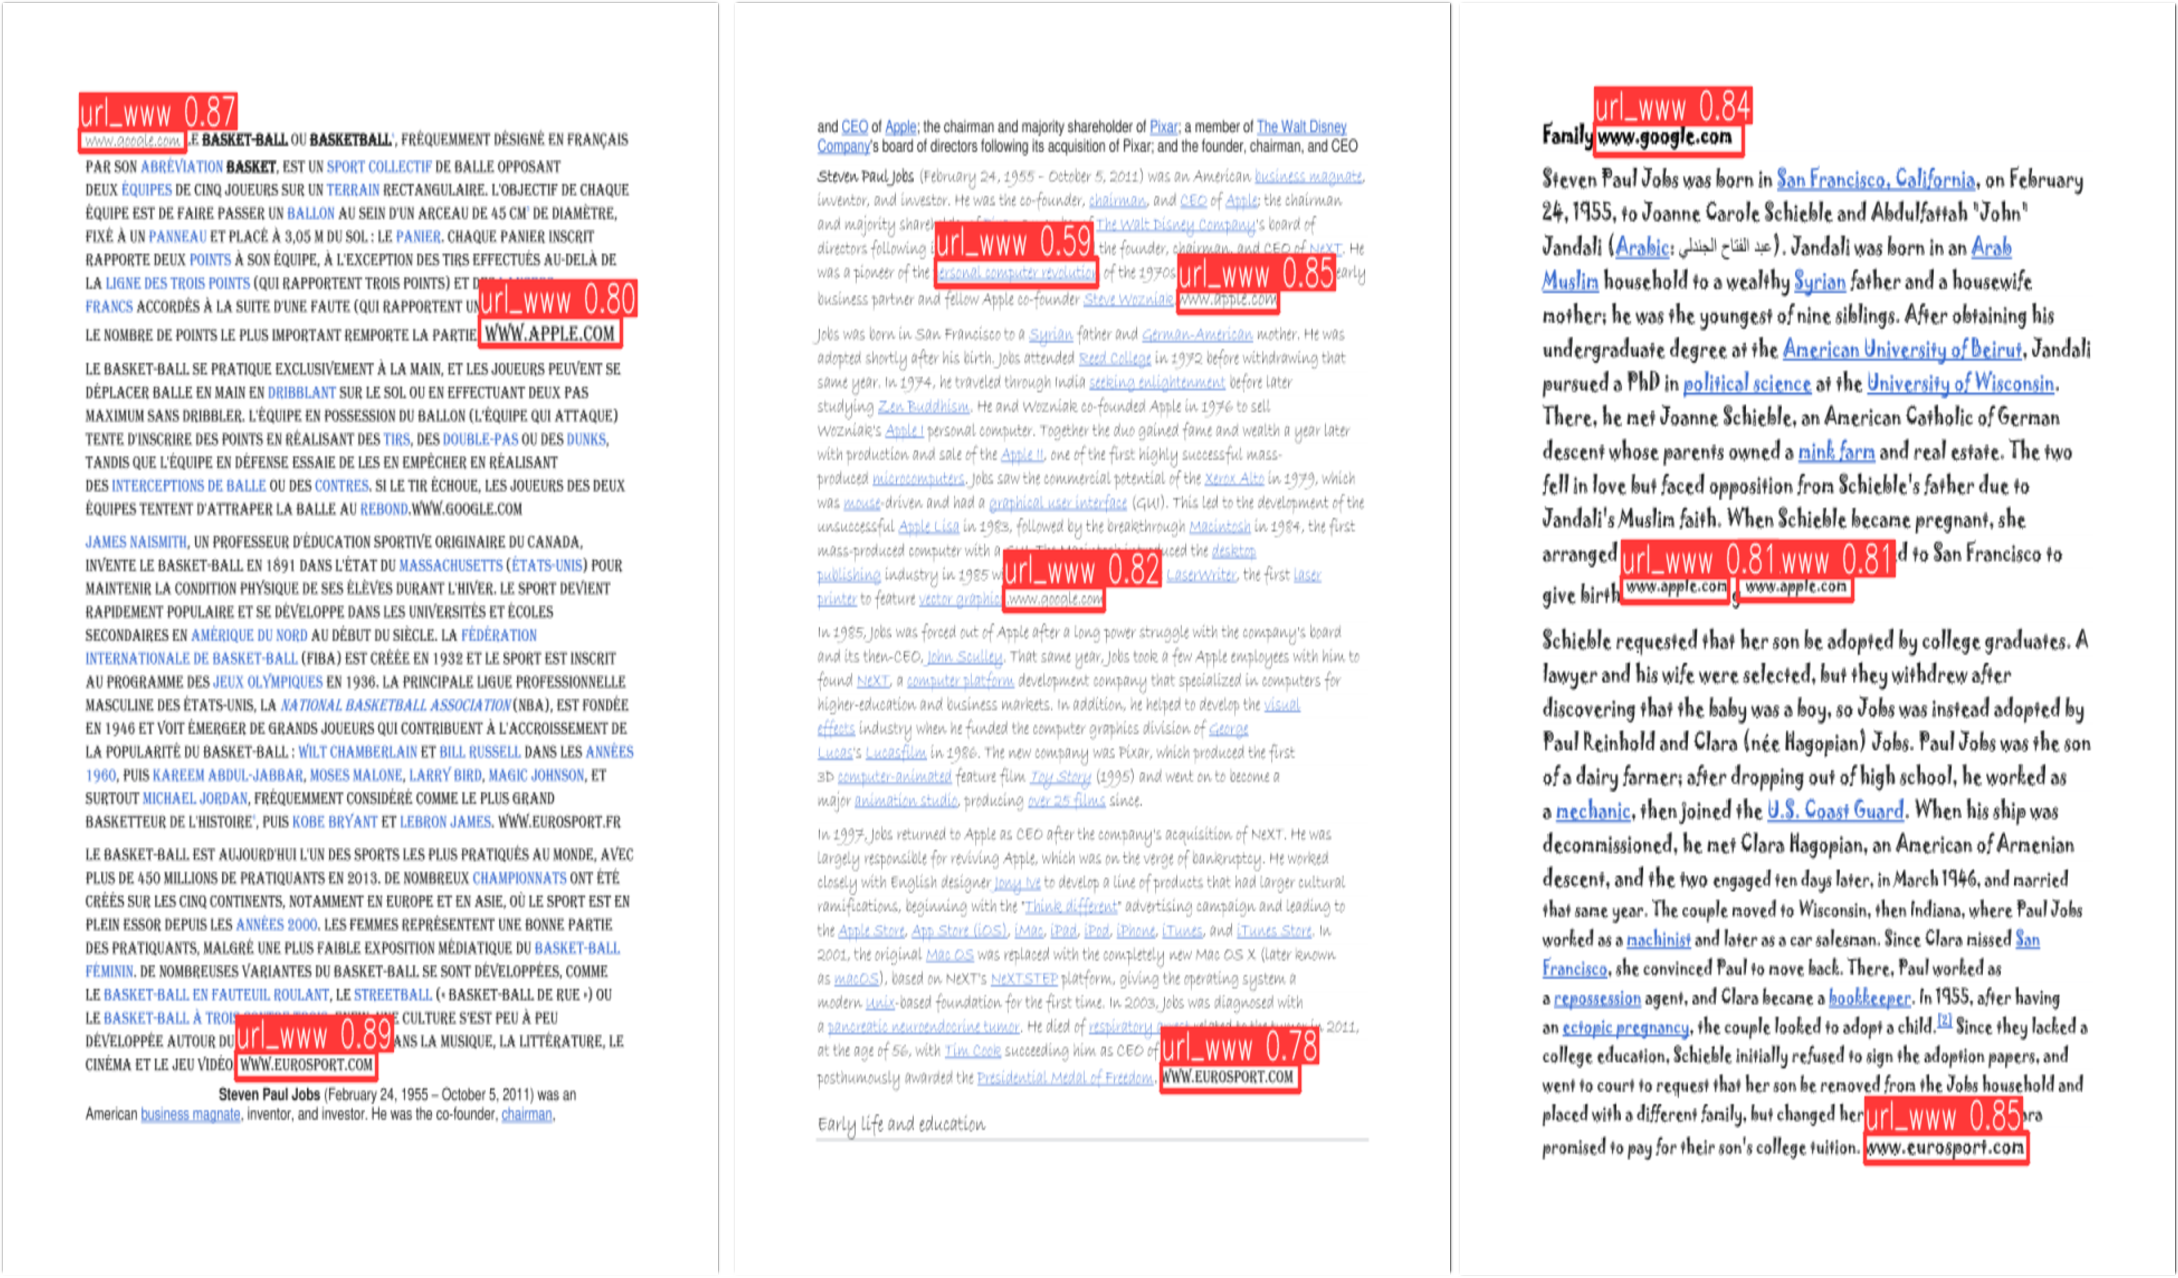
\includegraphics[height=9cm,width=17cm]{Chapitre3/font_yolov5.png}
                    \caption{Test de difficulté: Différentes polices de caractères - YOLOv5.}
                    \label{y5_t2}
                    \end{figure}

          % ---------- COLOR --------------
          \subsubsection{Différentes couleurs de fond et couleurs de caractères}
          Cette difficulté a fortement affecté les performances des modèles,
          YOLOv3 n'est pas capable de détecter les URL avec une couleur de fond colorée mais réussit à détecter les URL avec des caractères colorés, le modèle a obtenu $31,71\%$ de précision moyenne.
          YOLOv4 est le modèle performant dans cette difficulté avec une précision moyenne de $54,44\%$, il a réussi à détecter toutes les URL avec des caractères colorés et la plupart des URL avec un fond coloré.
          YOLOv5 est le moins performant de tous avec une précision moyenne de $27,27\%$ où il ne peut pas détecter complètement les URL avec des objets colorés et encore moins des arrière-plans colorés
          \begin{figure}[H]
               \centering
                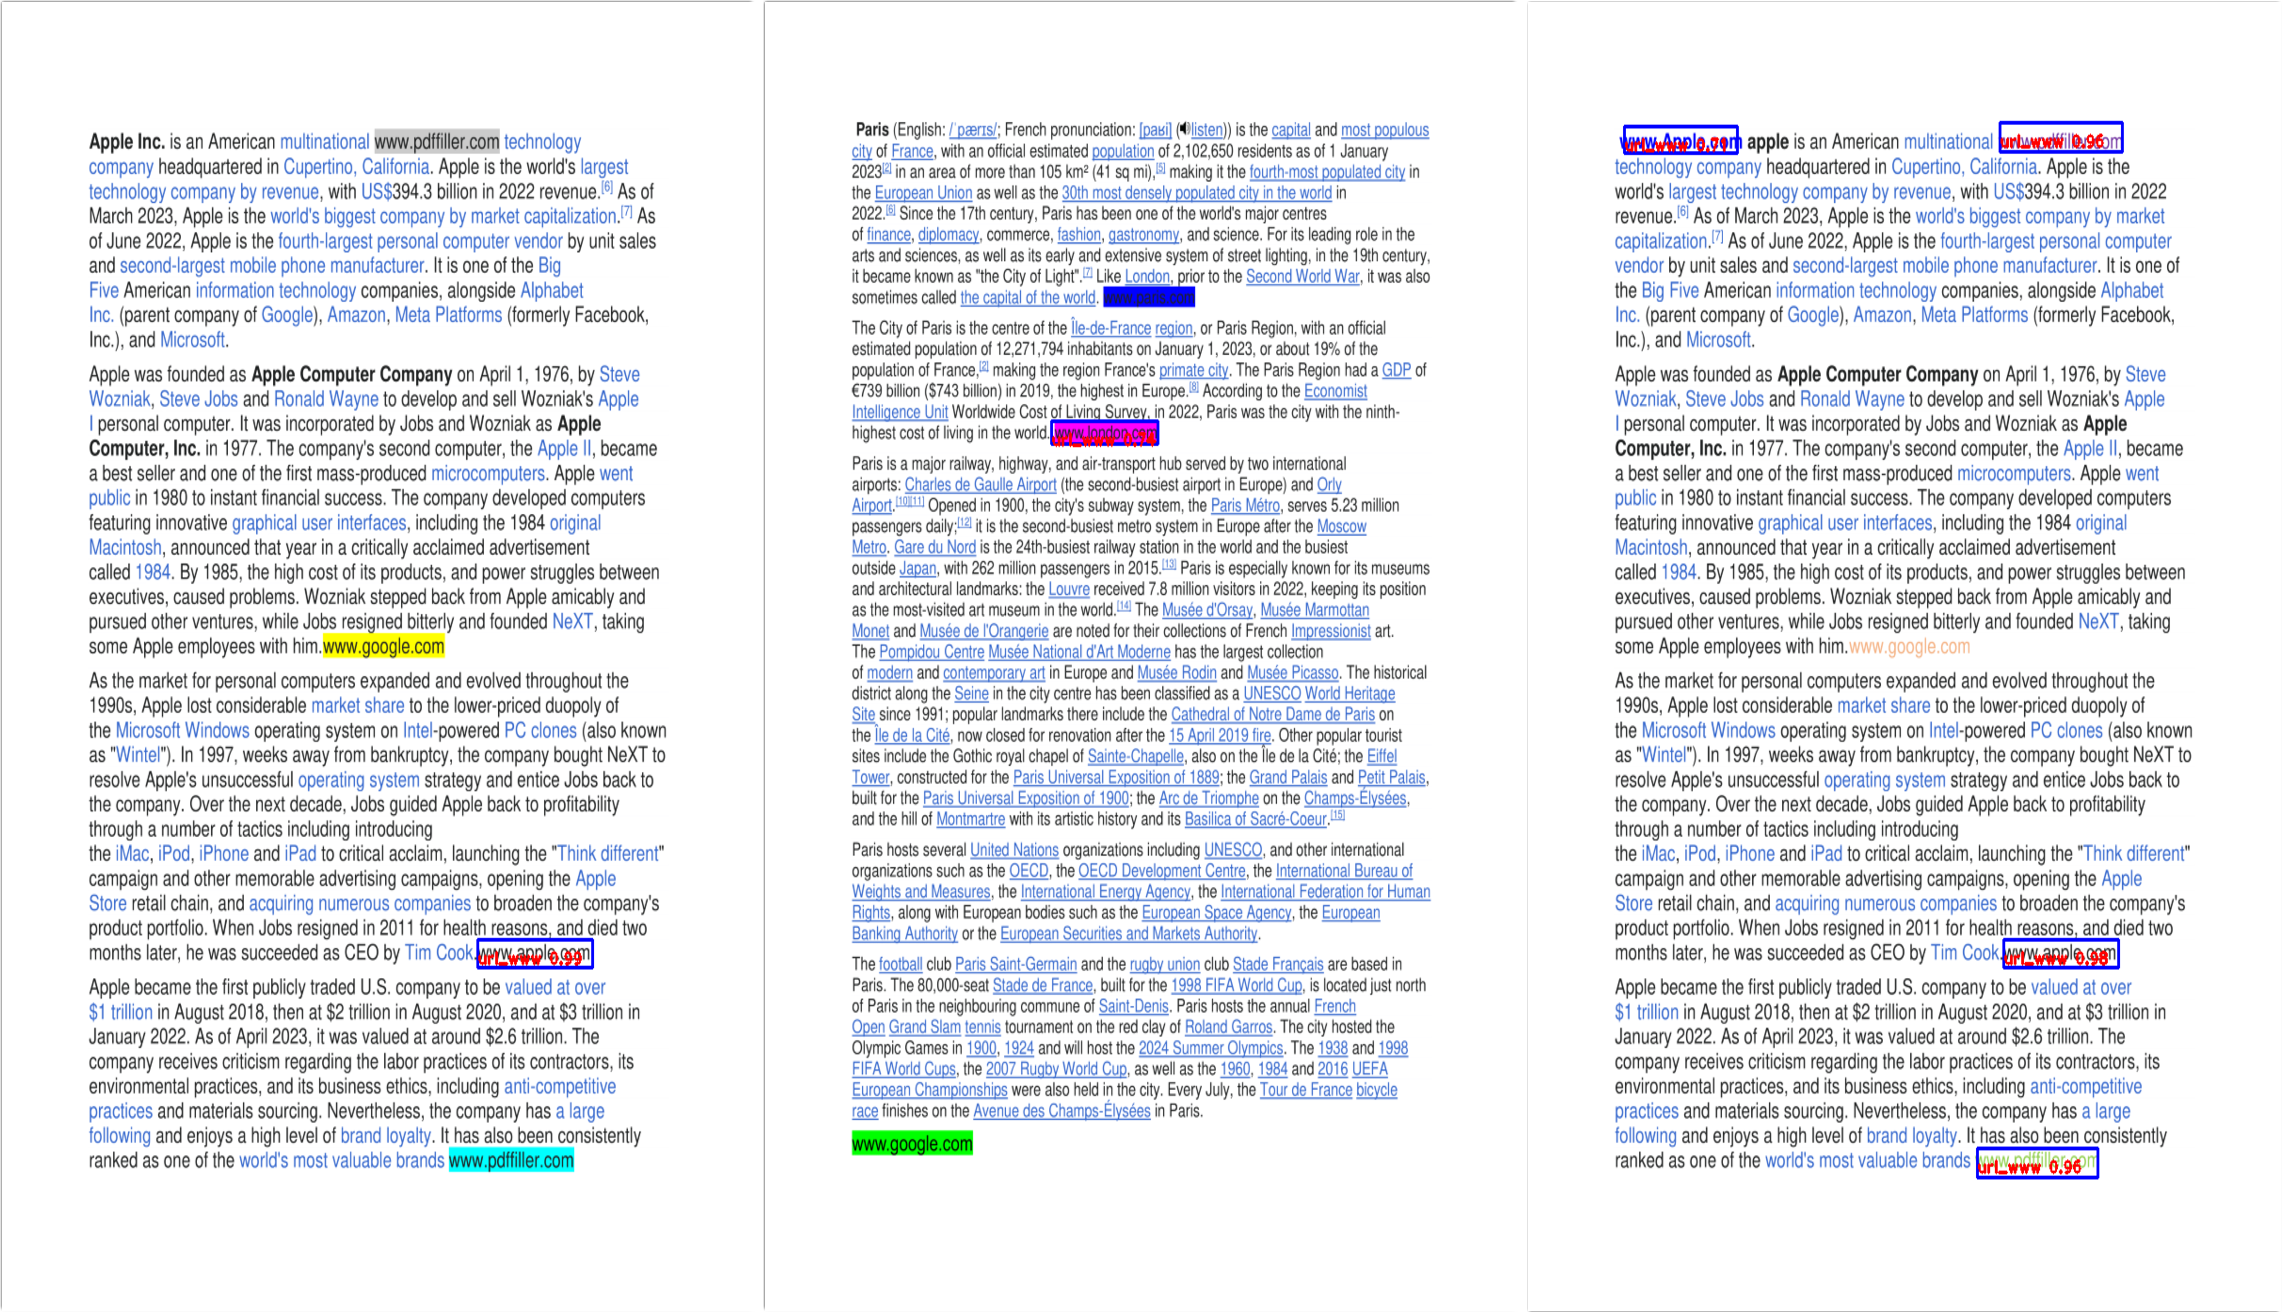
\includegraphics[height=9cm,width=17cm]{Chapitre3/color_yolov3.png}
                \caption{Test de difficulté: Différentes couleurs de fond et couleurs de caractères - YOLOv3.}
                \label{y3_t3}
                \end{figure}
          \begin{figure}[H]
                    \centering
                    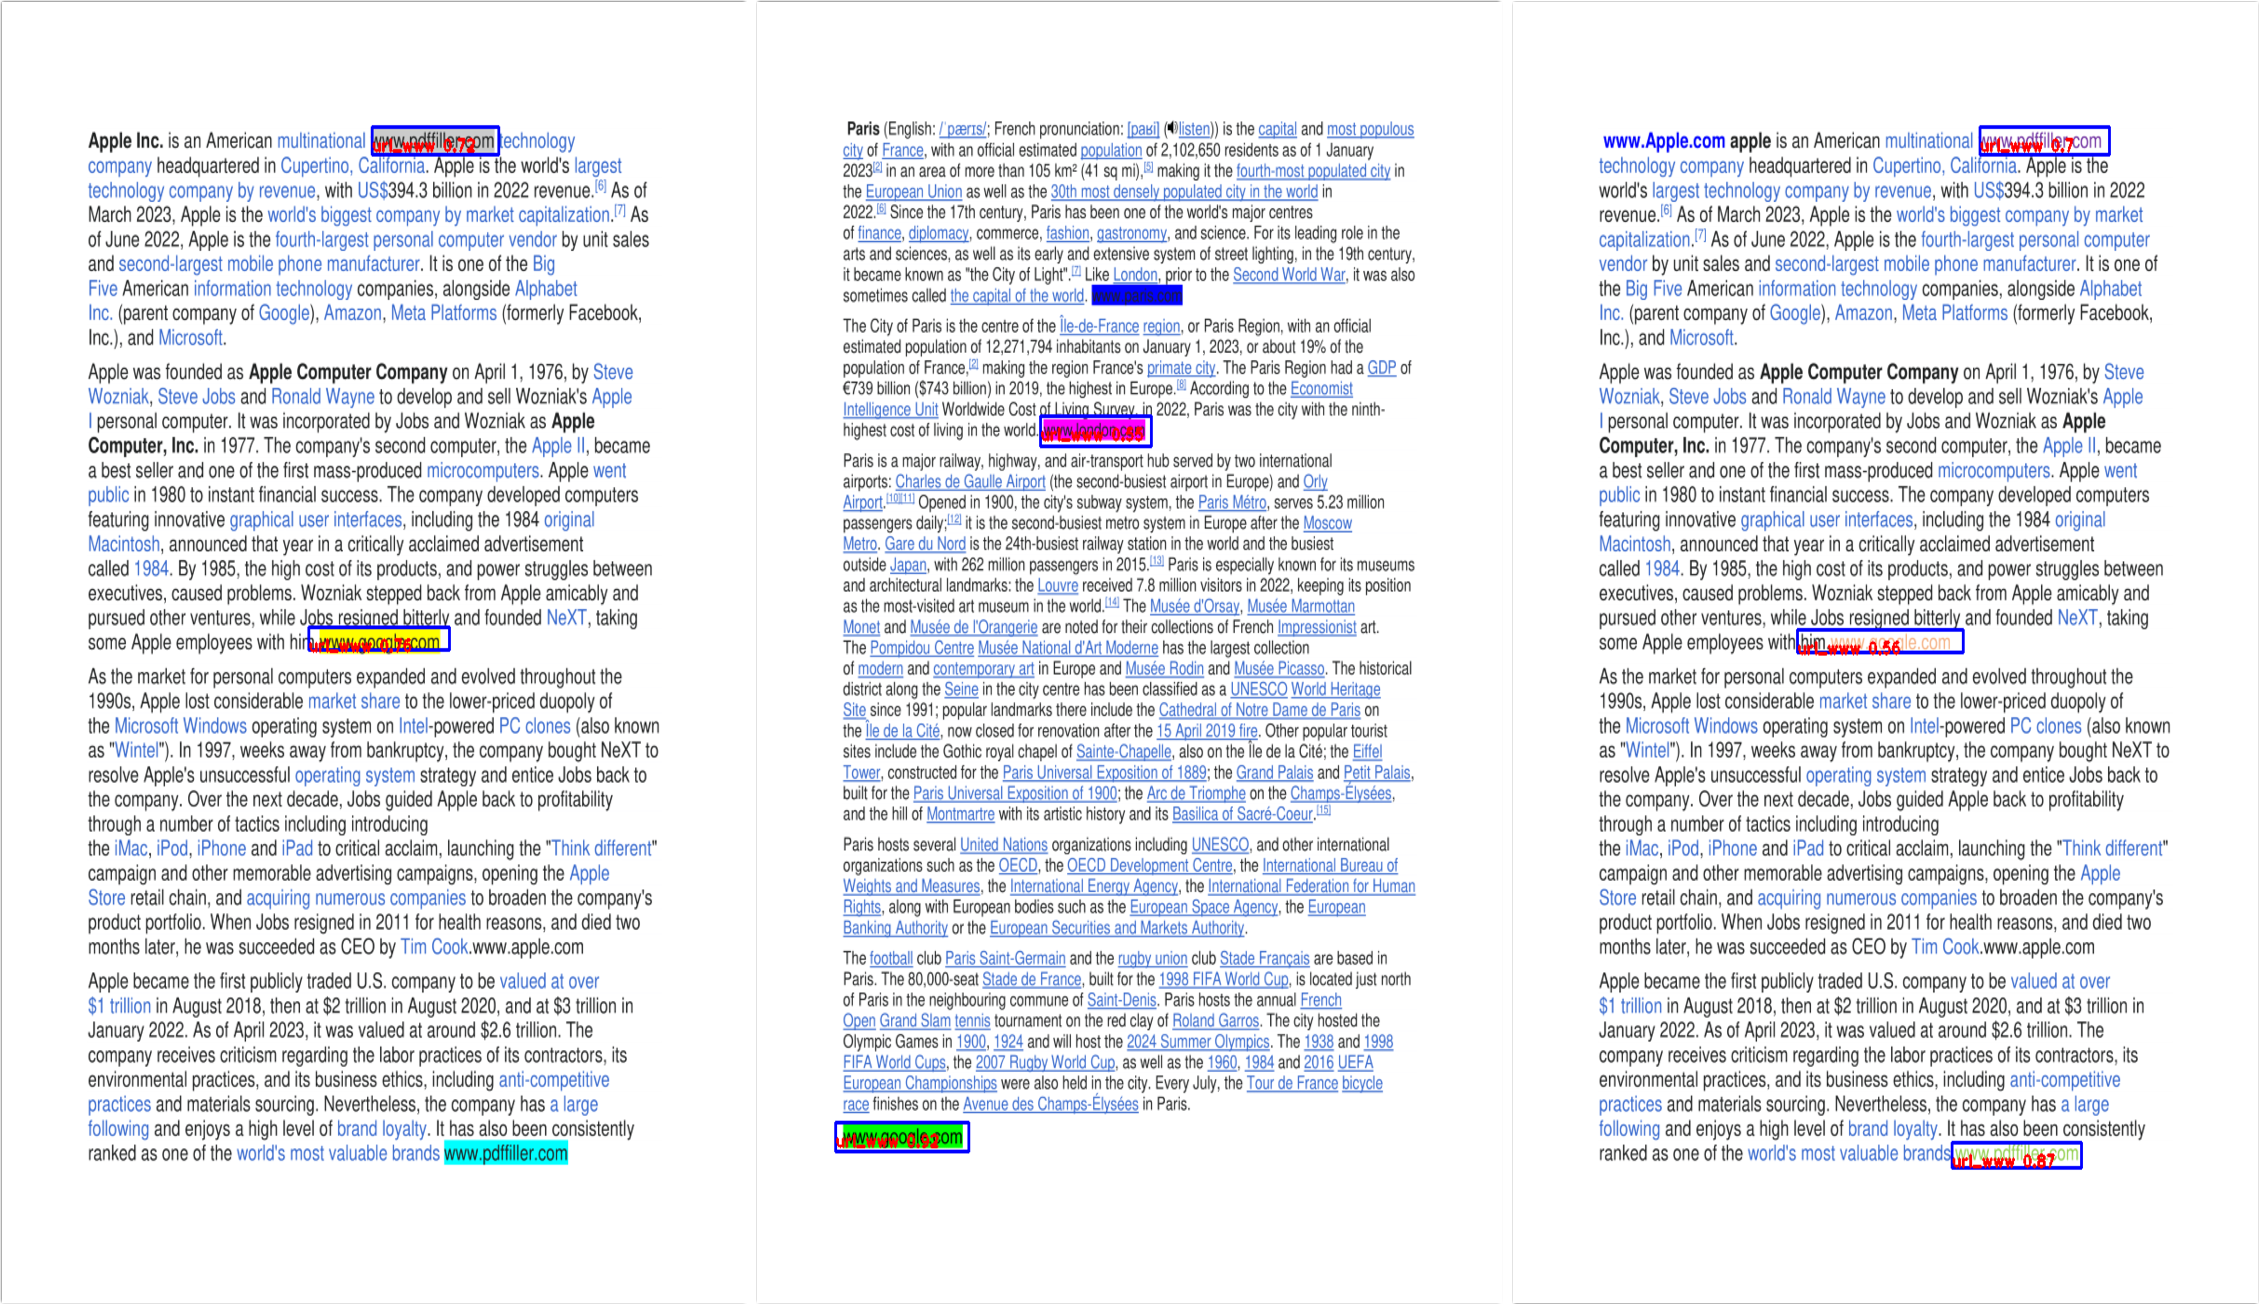
\includegraphics[height=9cm,width=17cm]{Chapitre3/color_yolov4.png}
                    \caption{Test de difficulté: Différentes couleurs de fond et couleurs de caractères - YOLOv4.}
                    \label{y4_t3}
                    \end{figure}
          \begin{figure}[H]
                    \centering
                    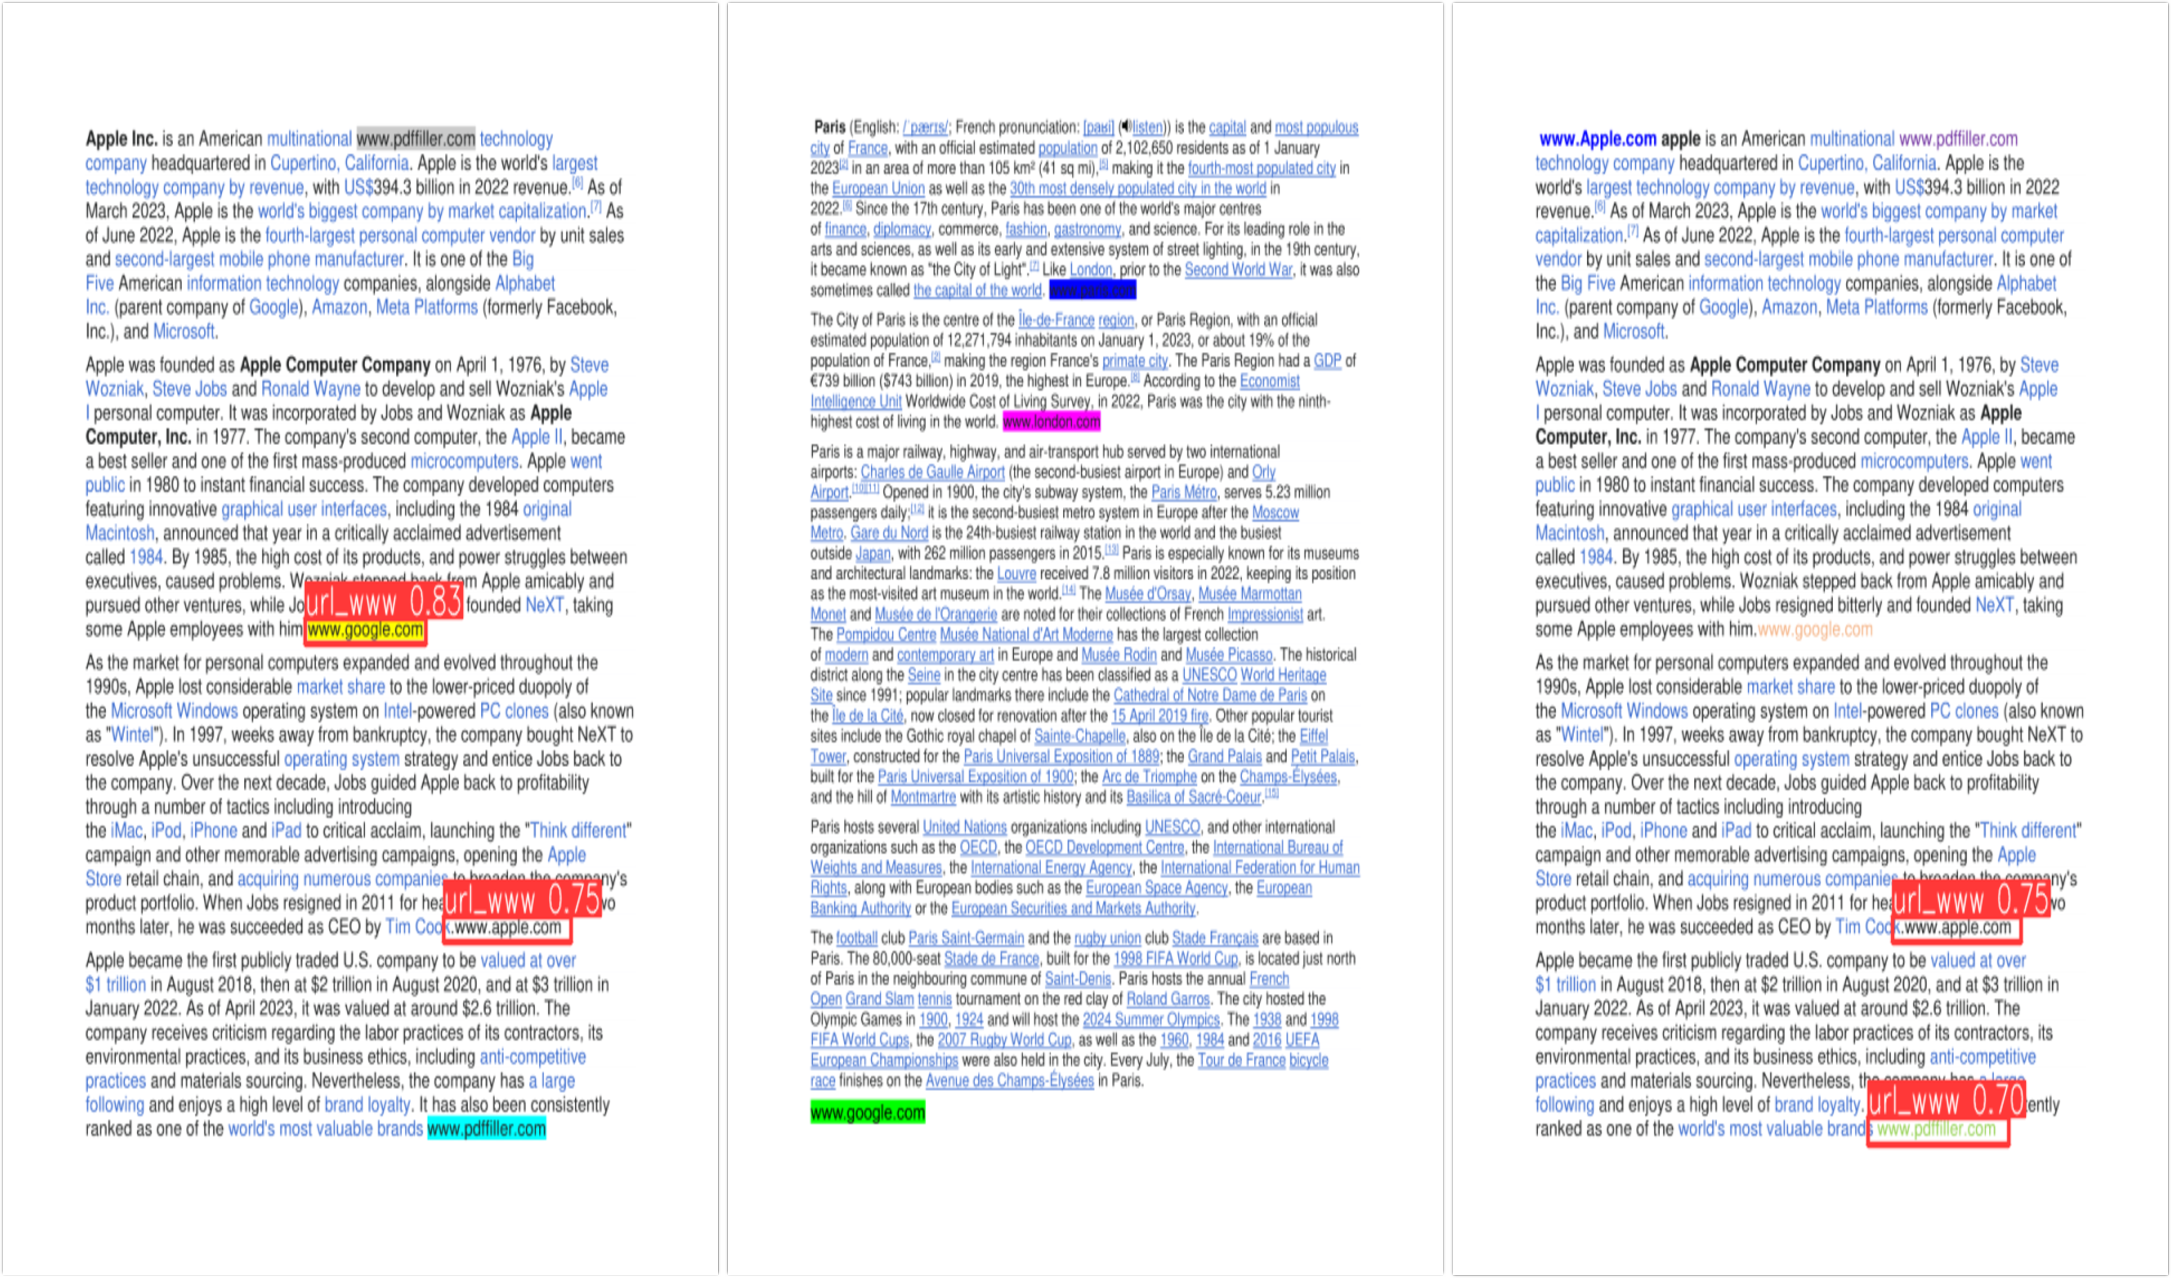
\includegraphics[height=9cm,width=17cm]{Chapitre3/color_yolov5.png}
                    \caption{Test de difficulté: Différentes couleurs de fond et couleurs de caractères - YOLOv5.}
                    \label{y5_t3}
                    \end{figure}
          
          % ---------- ROTATION --------------
          \subsubsection{Rotation des images sur $90^\circ$ et $180^\circ$}
          La rotation en $180^\circ$ n'a pas affecté les performances de tous les modèles comme cela ne s'est jamais produit. D'un autre côté, la rotation en $90\circ$ a totalement cassé les performances des modèles.
          \begin{figure}[H]
               \centering
                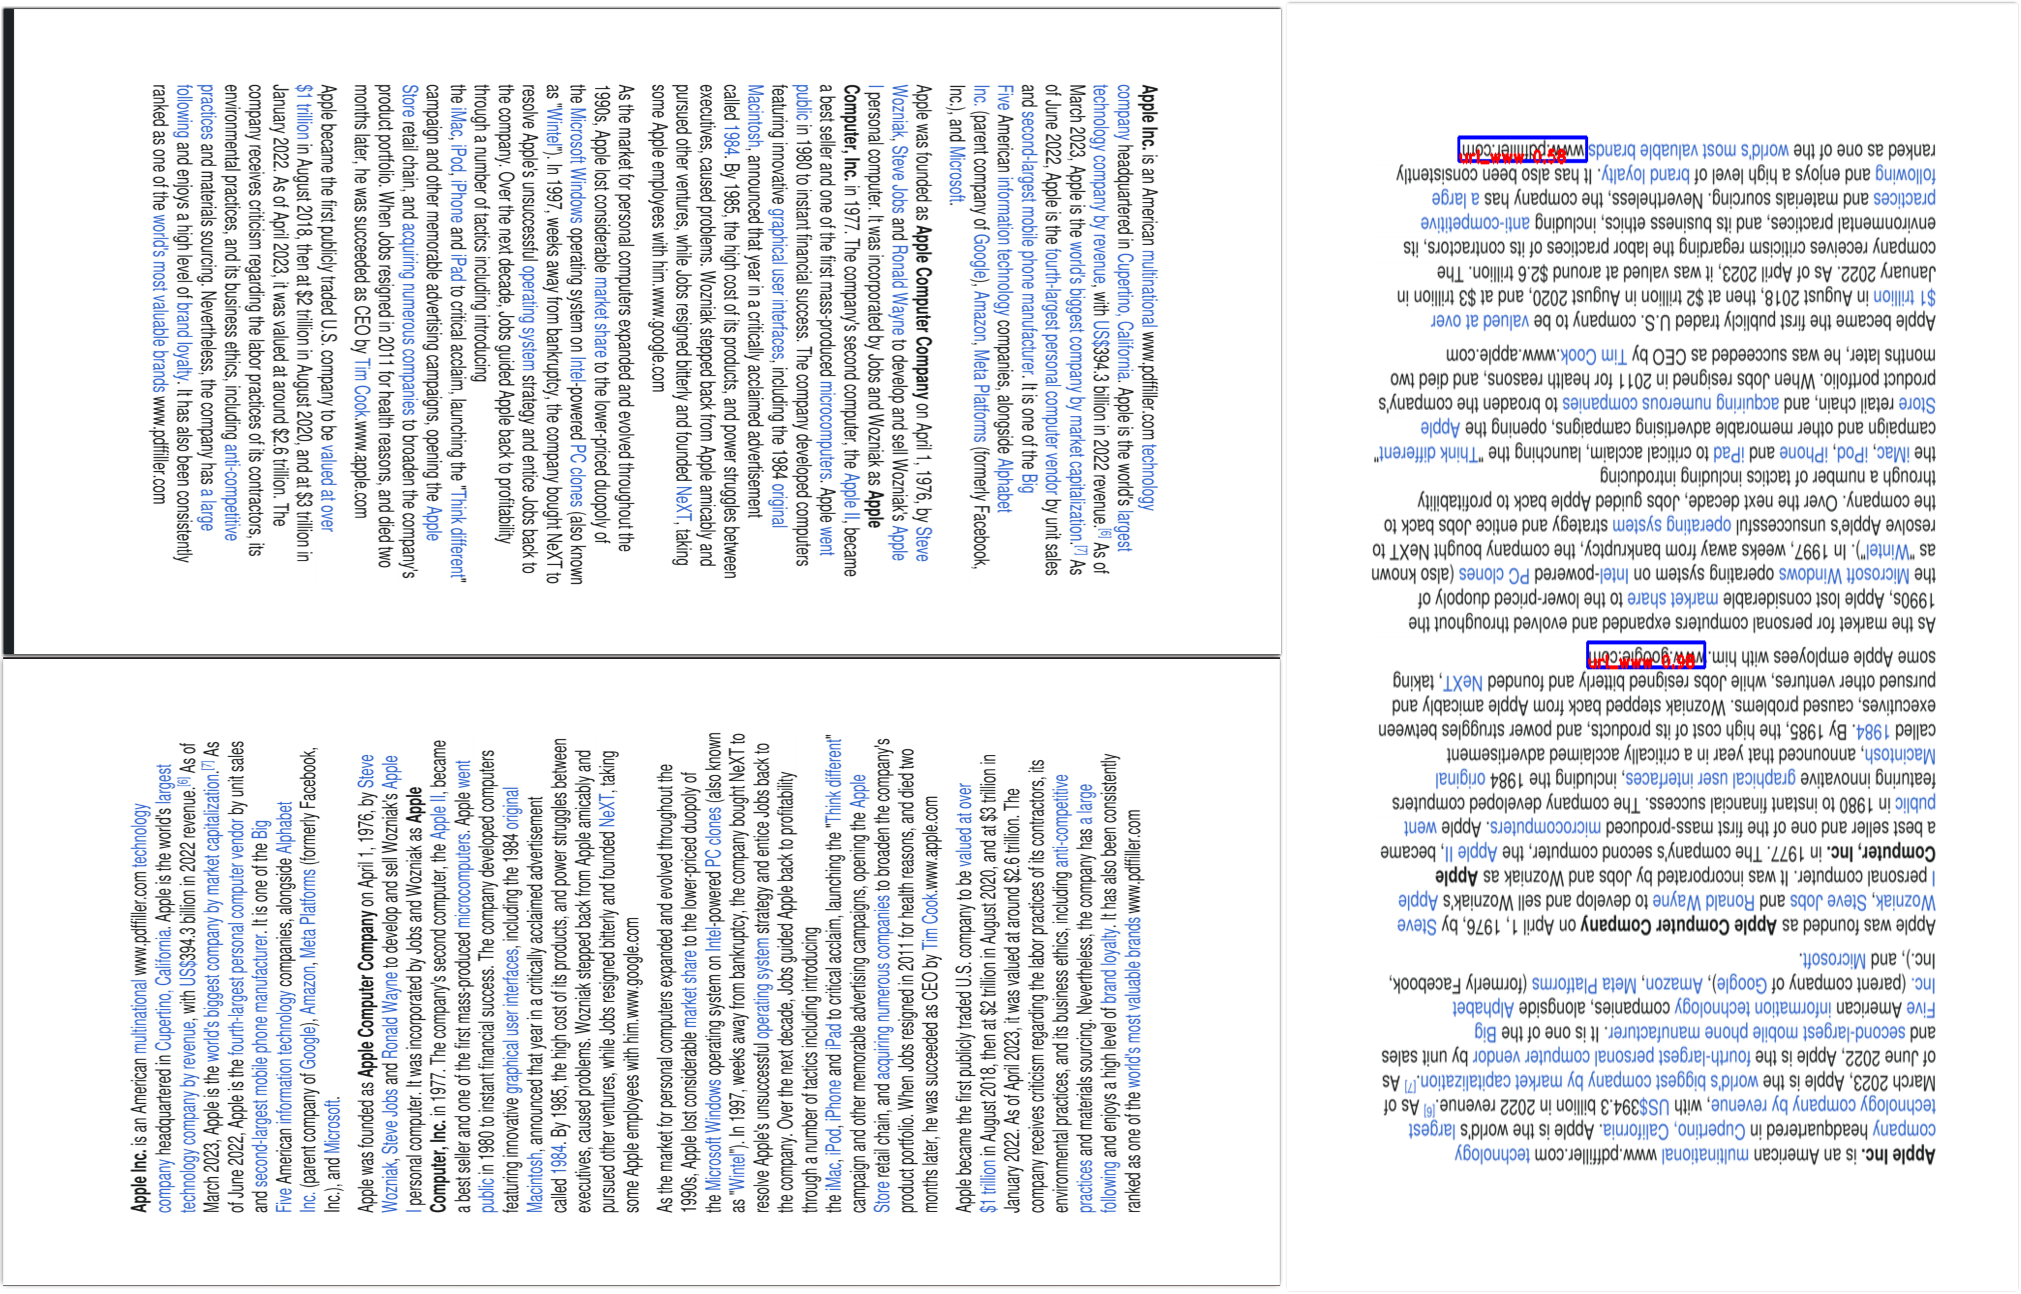
\includegraphics[height=12cm,width=17cm]{Chapitre3/rotation_yolov3.png}
                \caption{Test de difficulté: Rotation des images sur $90^\circ$ et $180^\circ$ - YOLOv3.}
                \label{y3_t5}
                \end{figure}
          \begin{figure}[H]
                    \centering
                    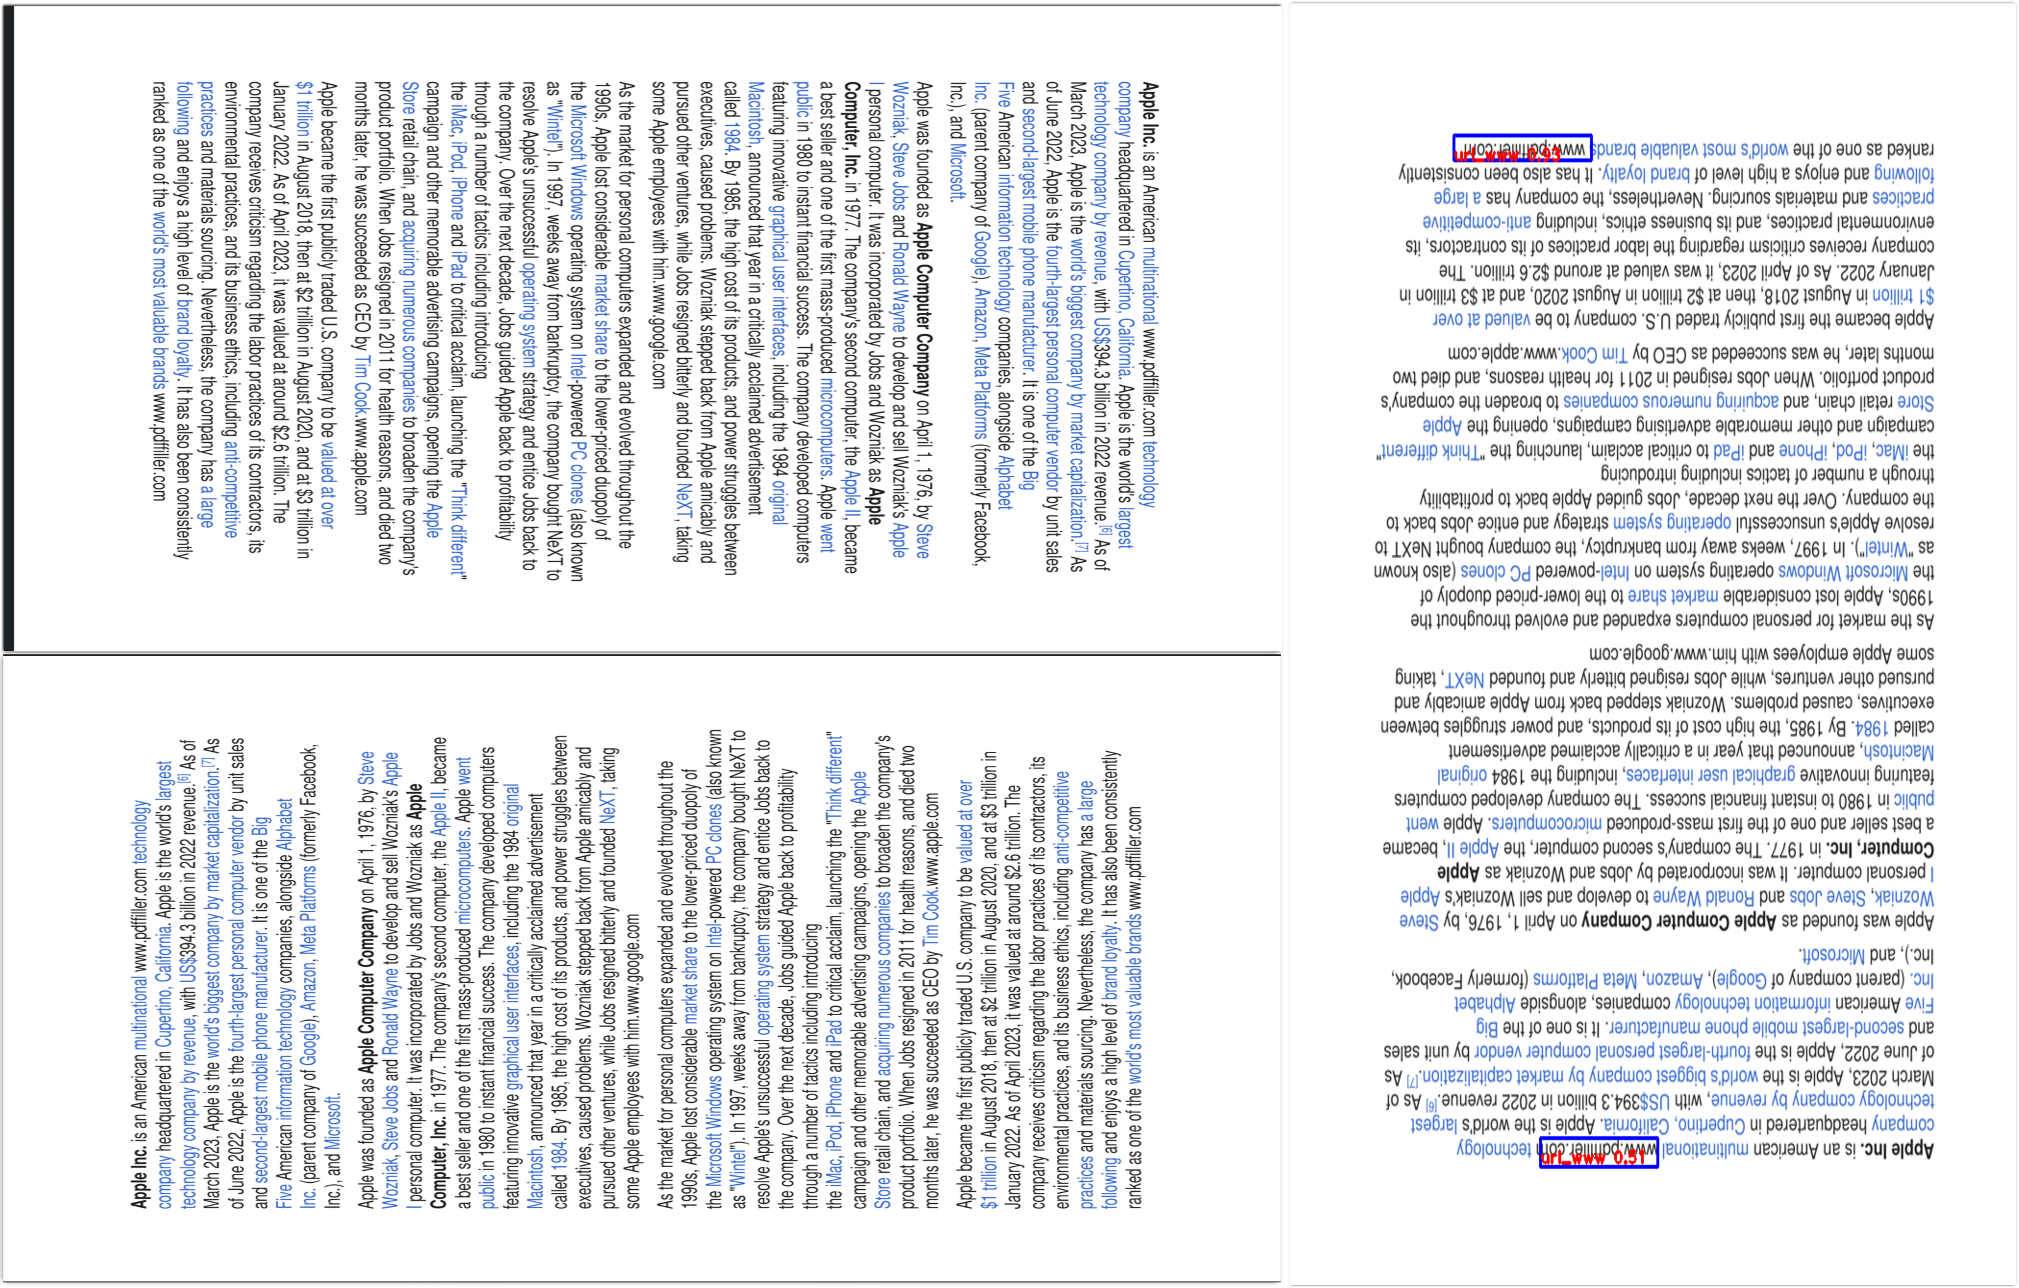
\includegraphics[height=12cm,width=17cm]{Chapitre3/rotation_yolov4.png}
                    \caption{Test de difficulté: Rotation des images sur $90^\circ$ et $180^\circ$ - YOLOv4.}
                    \label{y4_t4}
                    \end{figure}
          \begin{figure}[H]
                    \centering
                    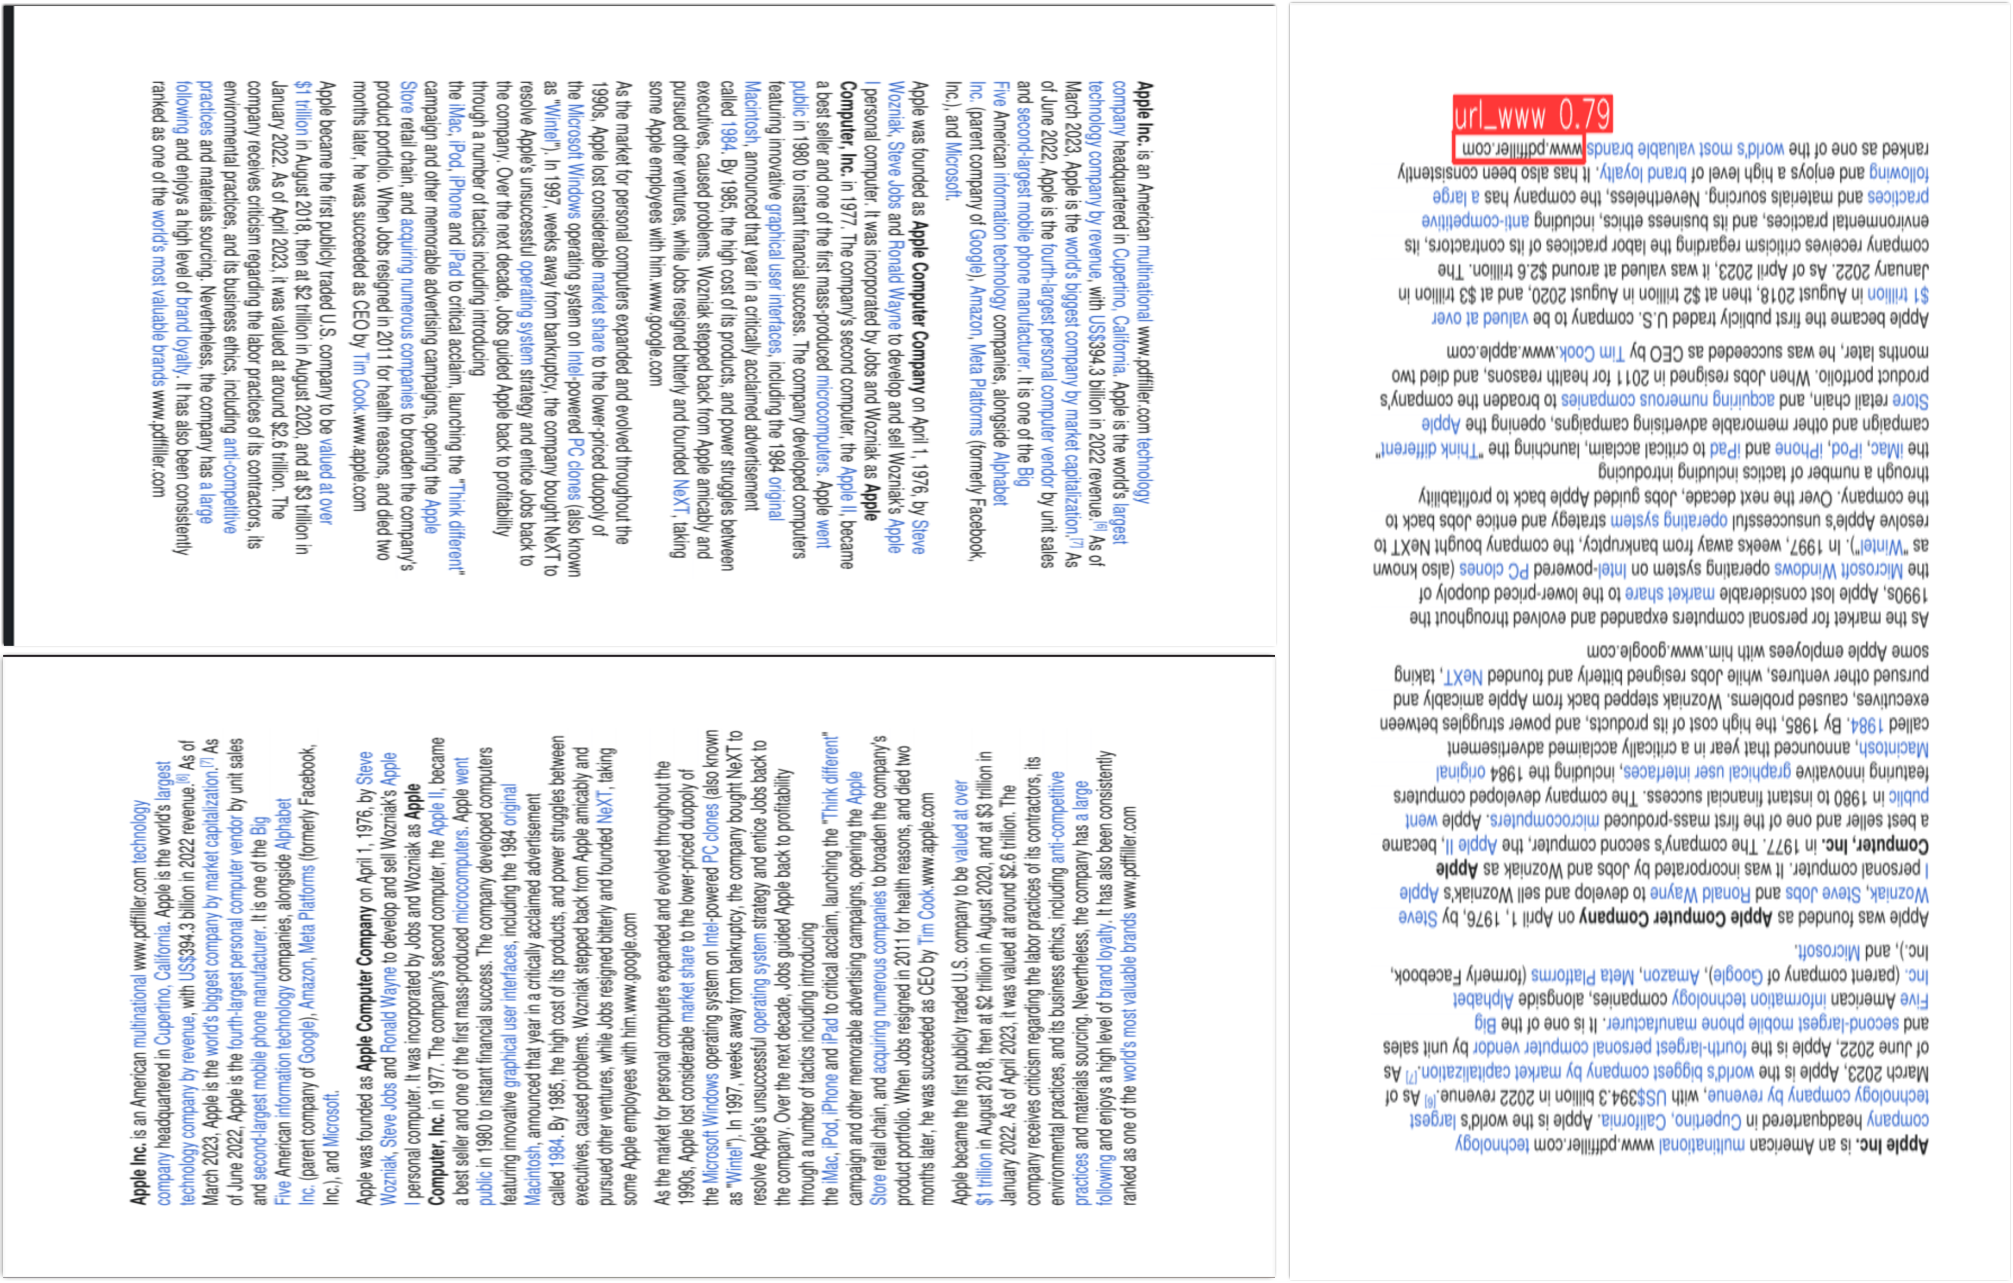
\includegraphics[height=12cm,width=17cm]{Chapitre3/rotation_yolov5.png}
                    \caption{Test de difficulté: Rotation des images sur $90^\circ$ et $180^\circ$ - YOLOv5.}
                    \label{y5_t4}
                    \end{figure}

          % ---------- PROTOCOL-TAG --------------  
          \subsubsection{URL préfixées avec la balise de protocole \textit{https://}}
          La plupart des URL, tous les modèles n'ont pas réussi à les détecter et certains n'ont pas détecté l'URL complète (de la balise de protocole à l'extension), mais ils n'ont détecté que le nom de domaine uniquement.
          YOLOv3 a obtenu un score de $12,12\%$, YOLOv4 avait la précision la plus élevée avec $28,9\%$ et YOLOv5 $13,64\%$.
          \begin{figure}[H]
               \centering
                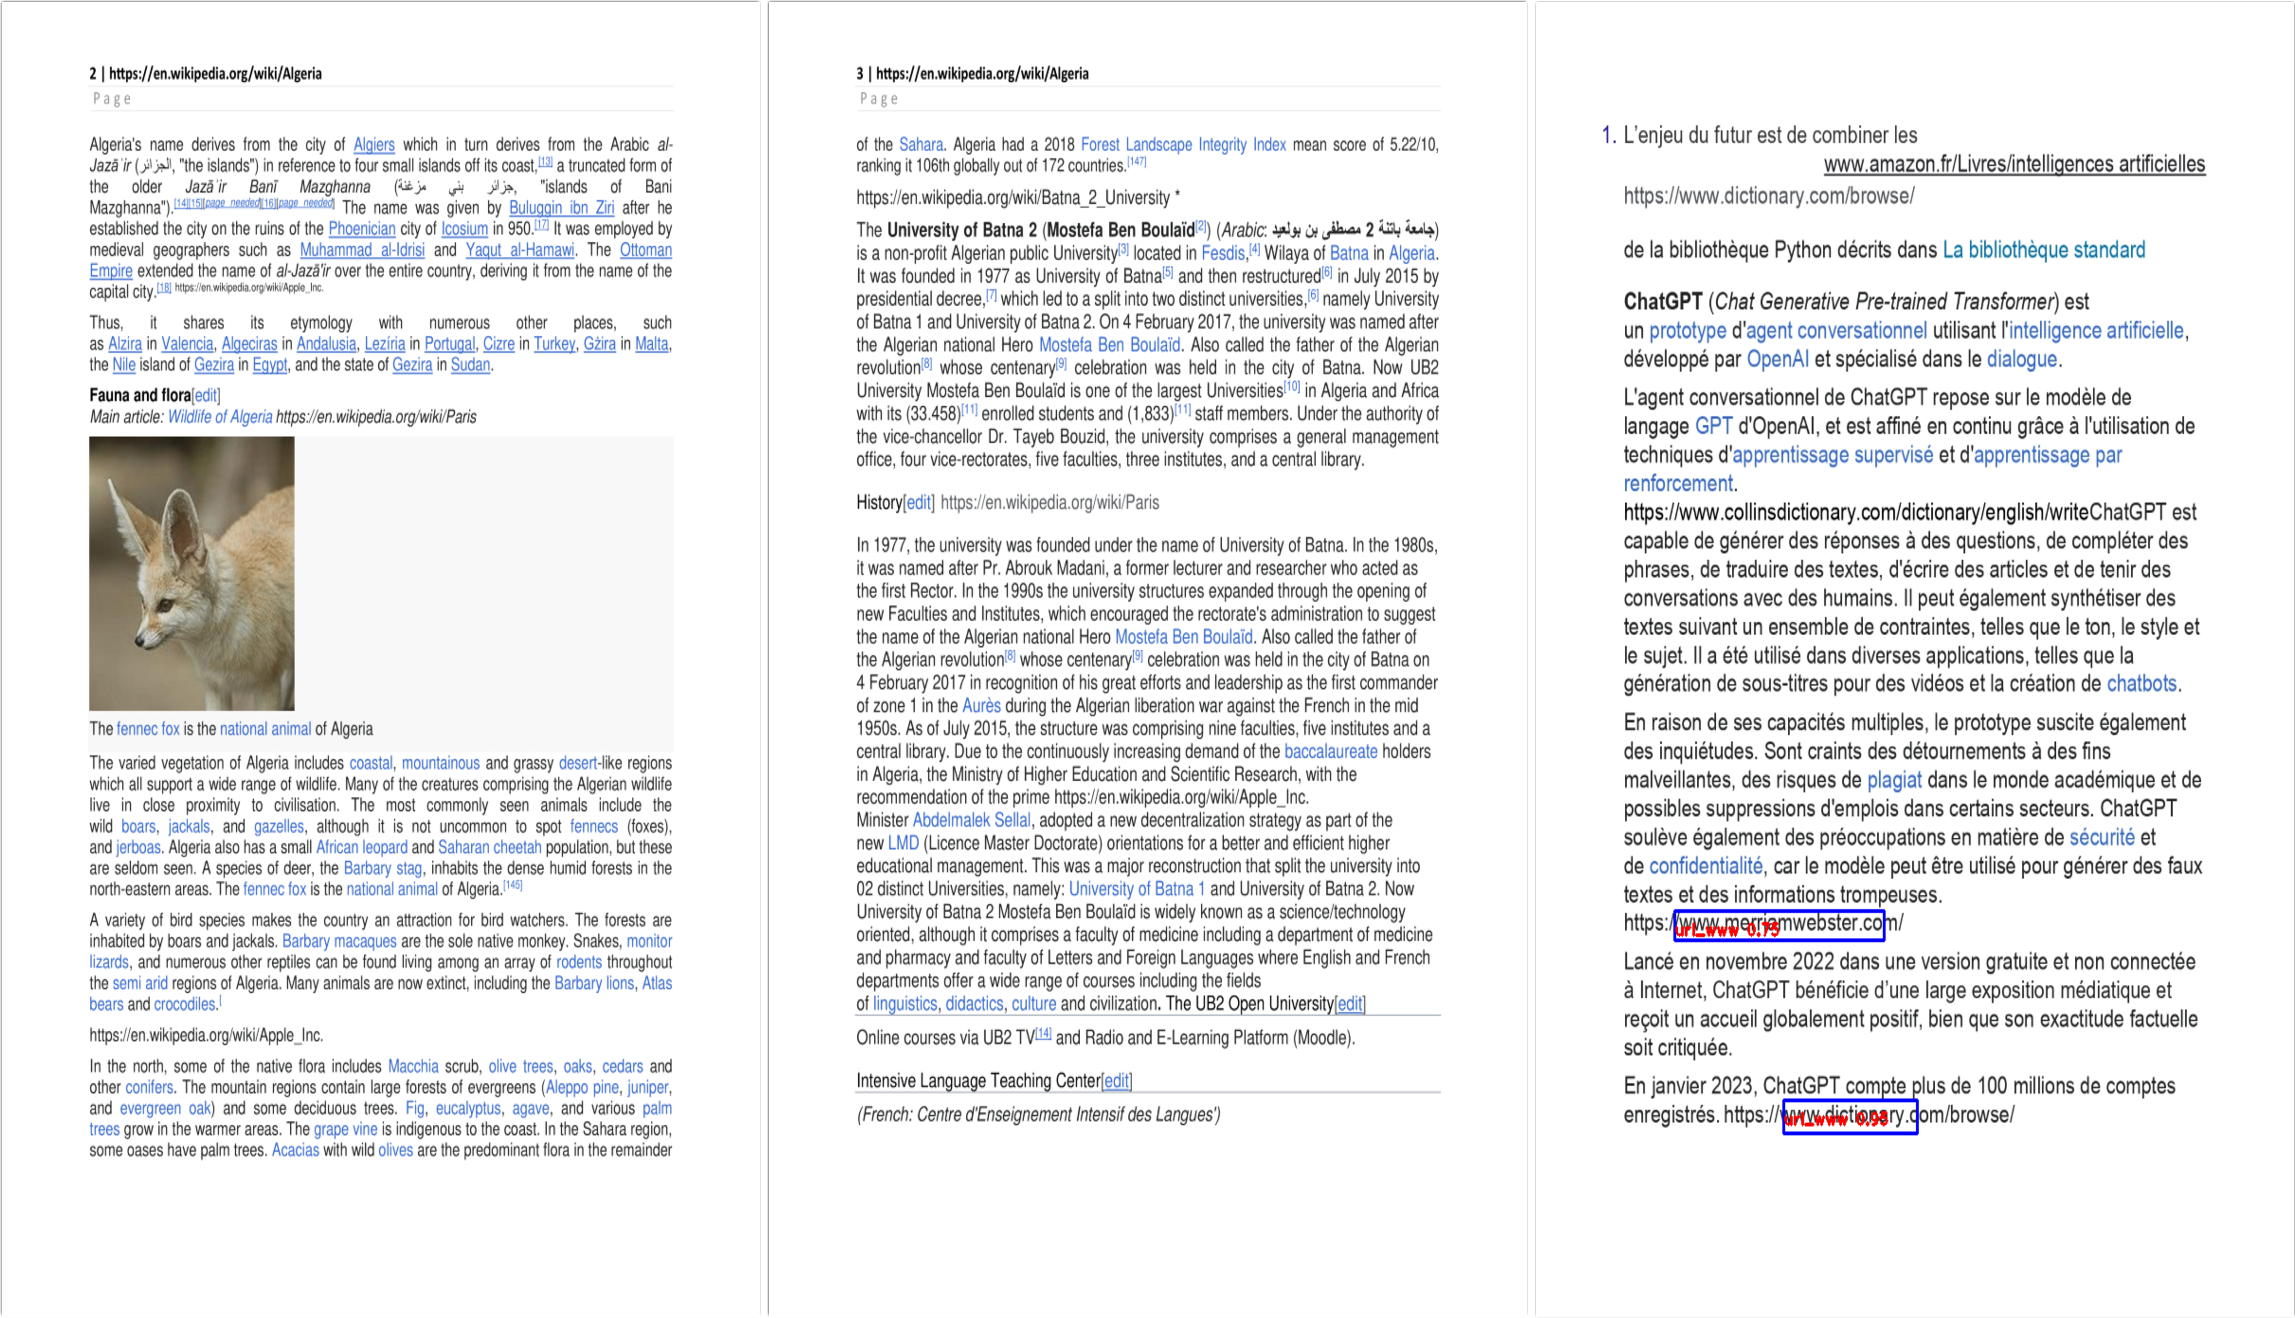
\includegraphics[height=9cm,width=17cm]{Chapitre3/https_yolov3.png}
                \caption{Test de difficulté: URL préfixées avec la balise de protocole \textit{https://} - YOLOv3.}
                \label{y3_t4}
                \end{figure}
          \begin{figure}[H]
                    \centering
                    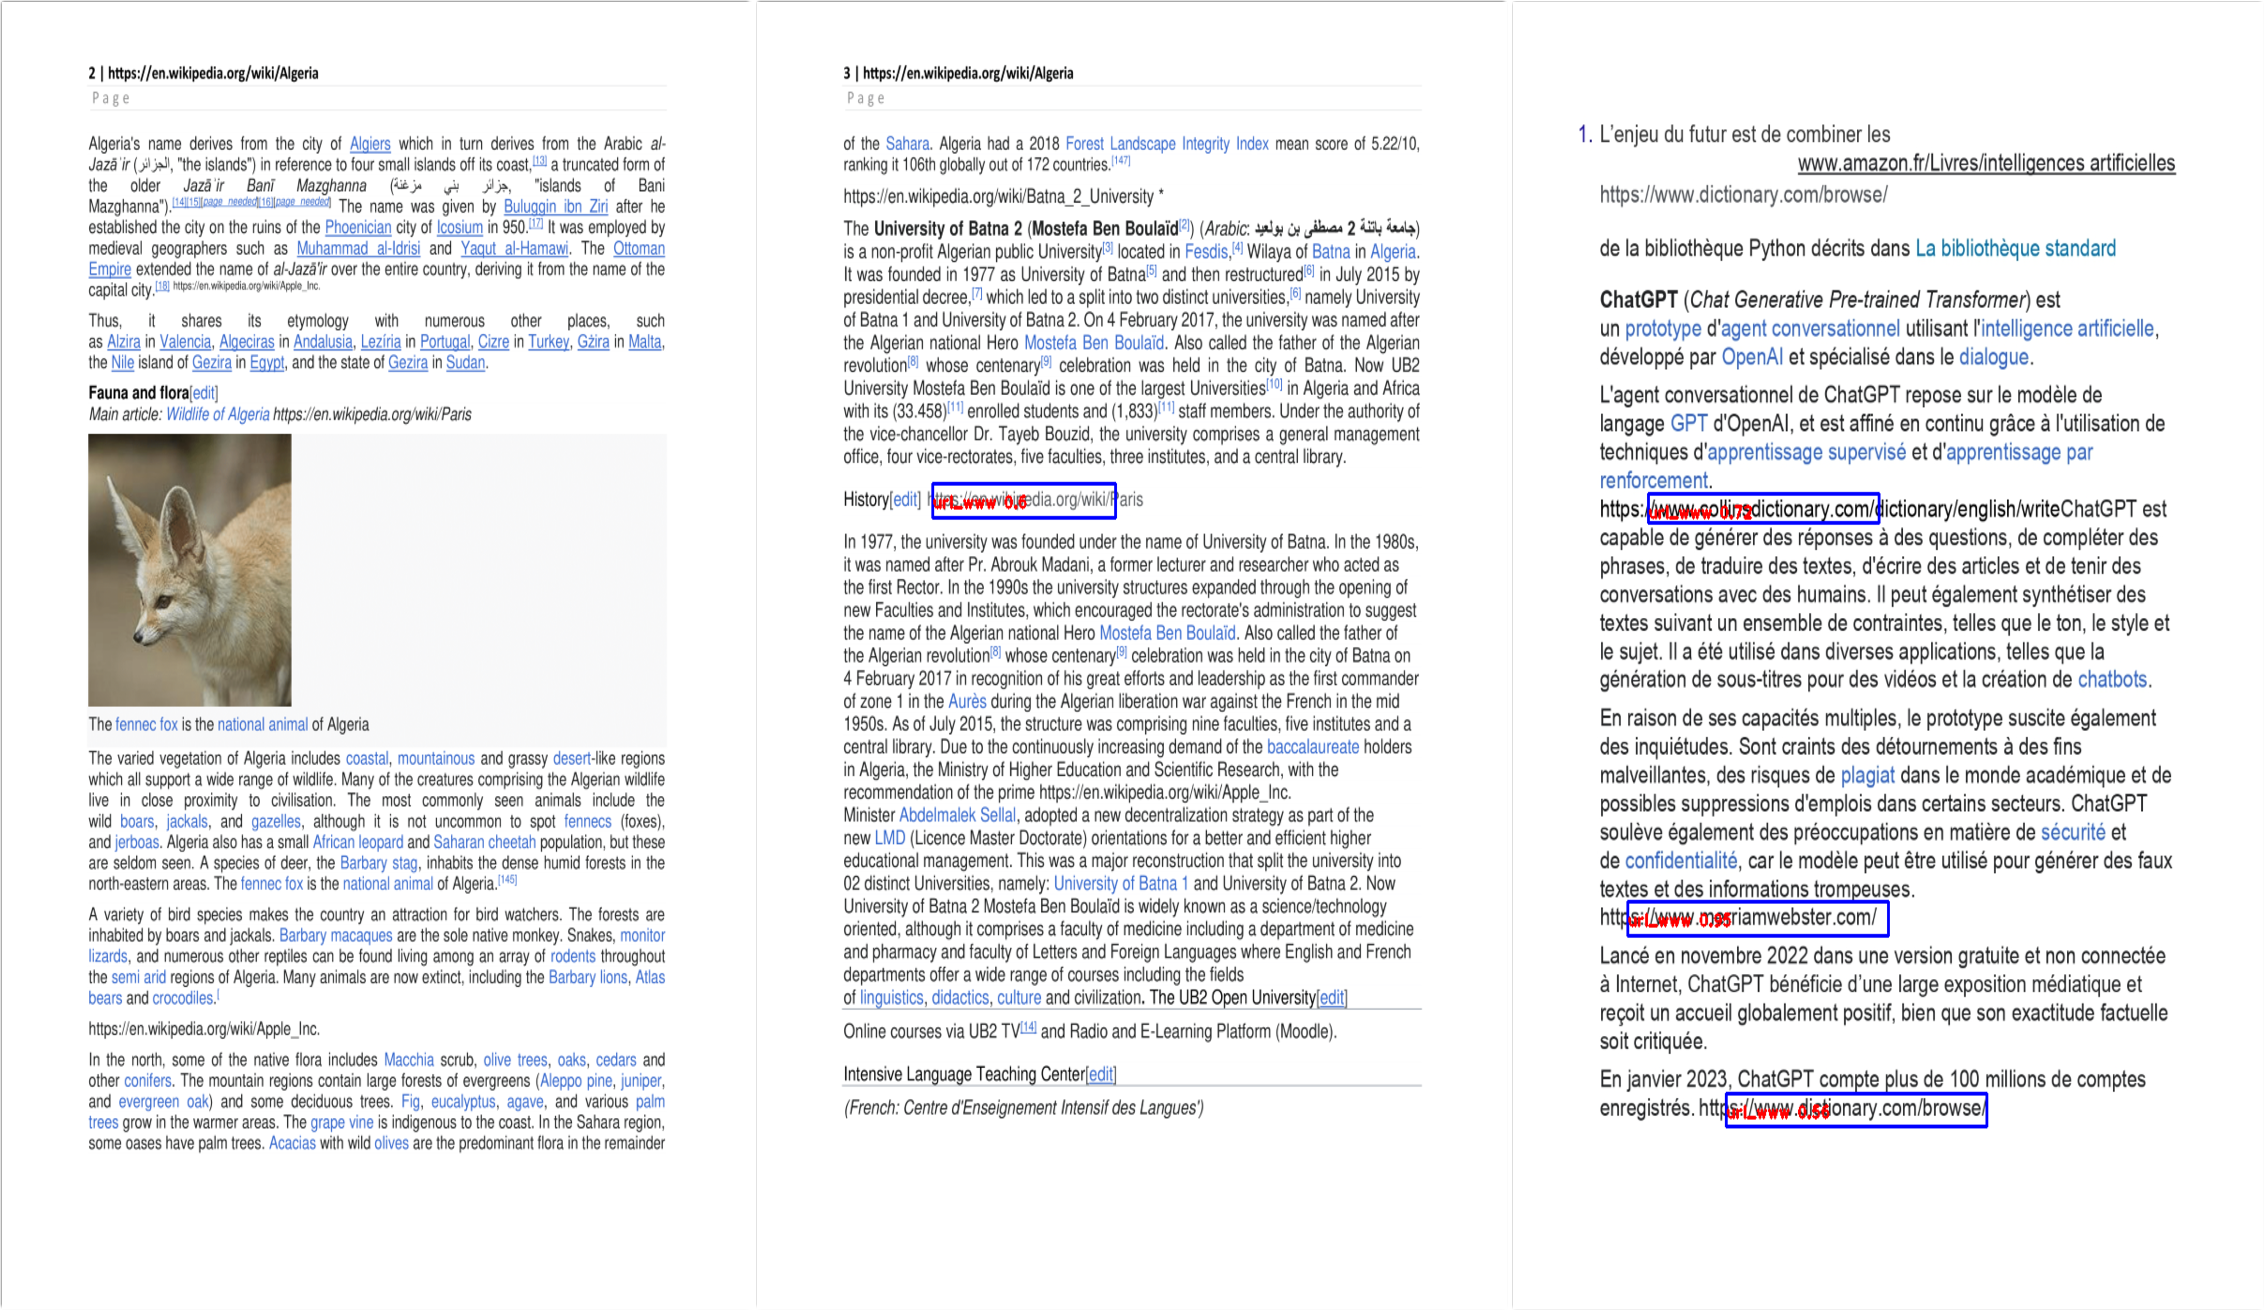
\includegraphics[height=9cm,width=17cm]{Chapitre3/https_yolov4.png}
                    \caption{Test de difficulté: URL préfixées avec la balise de protocole \textit{https://} - YOLOv4.}
                    \label{y4_https}
                    \end{figure}
          \begin{figure}[H]
                    \centering
                    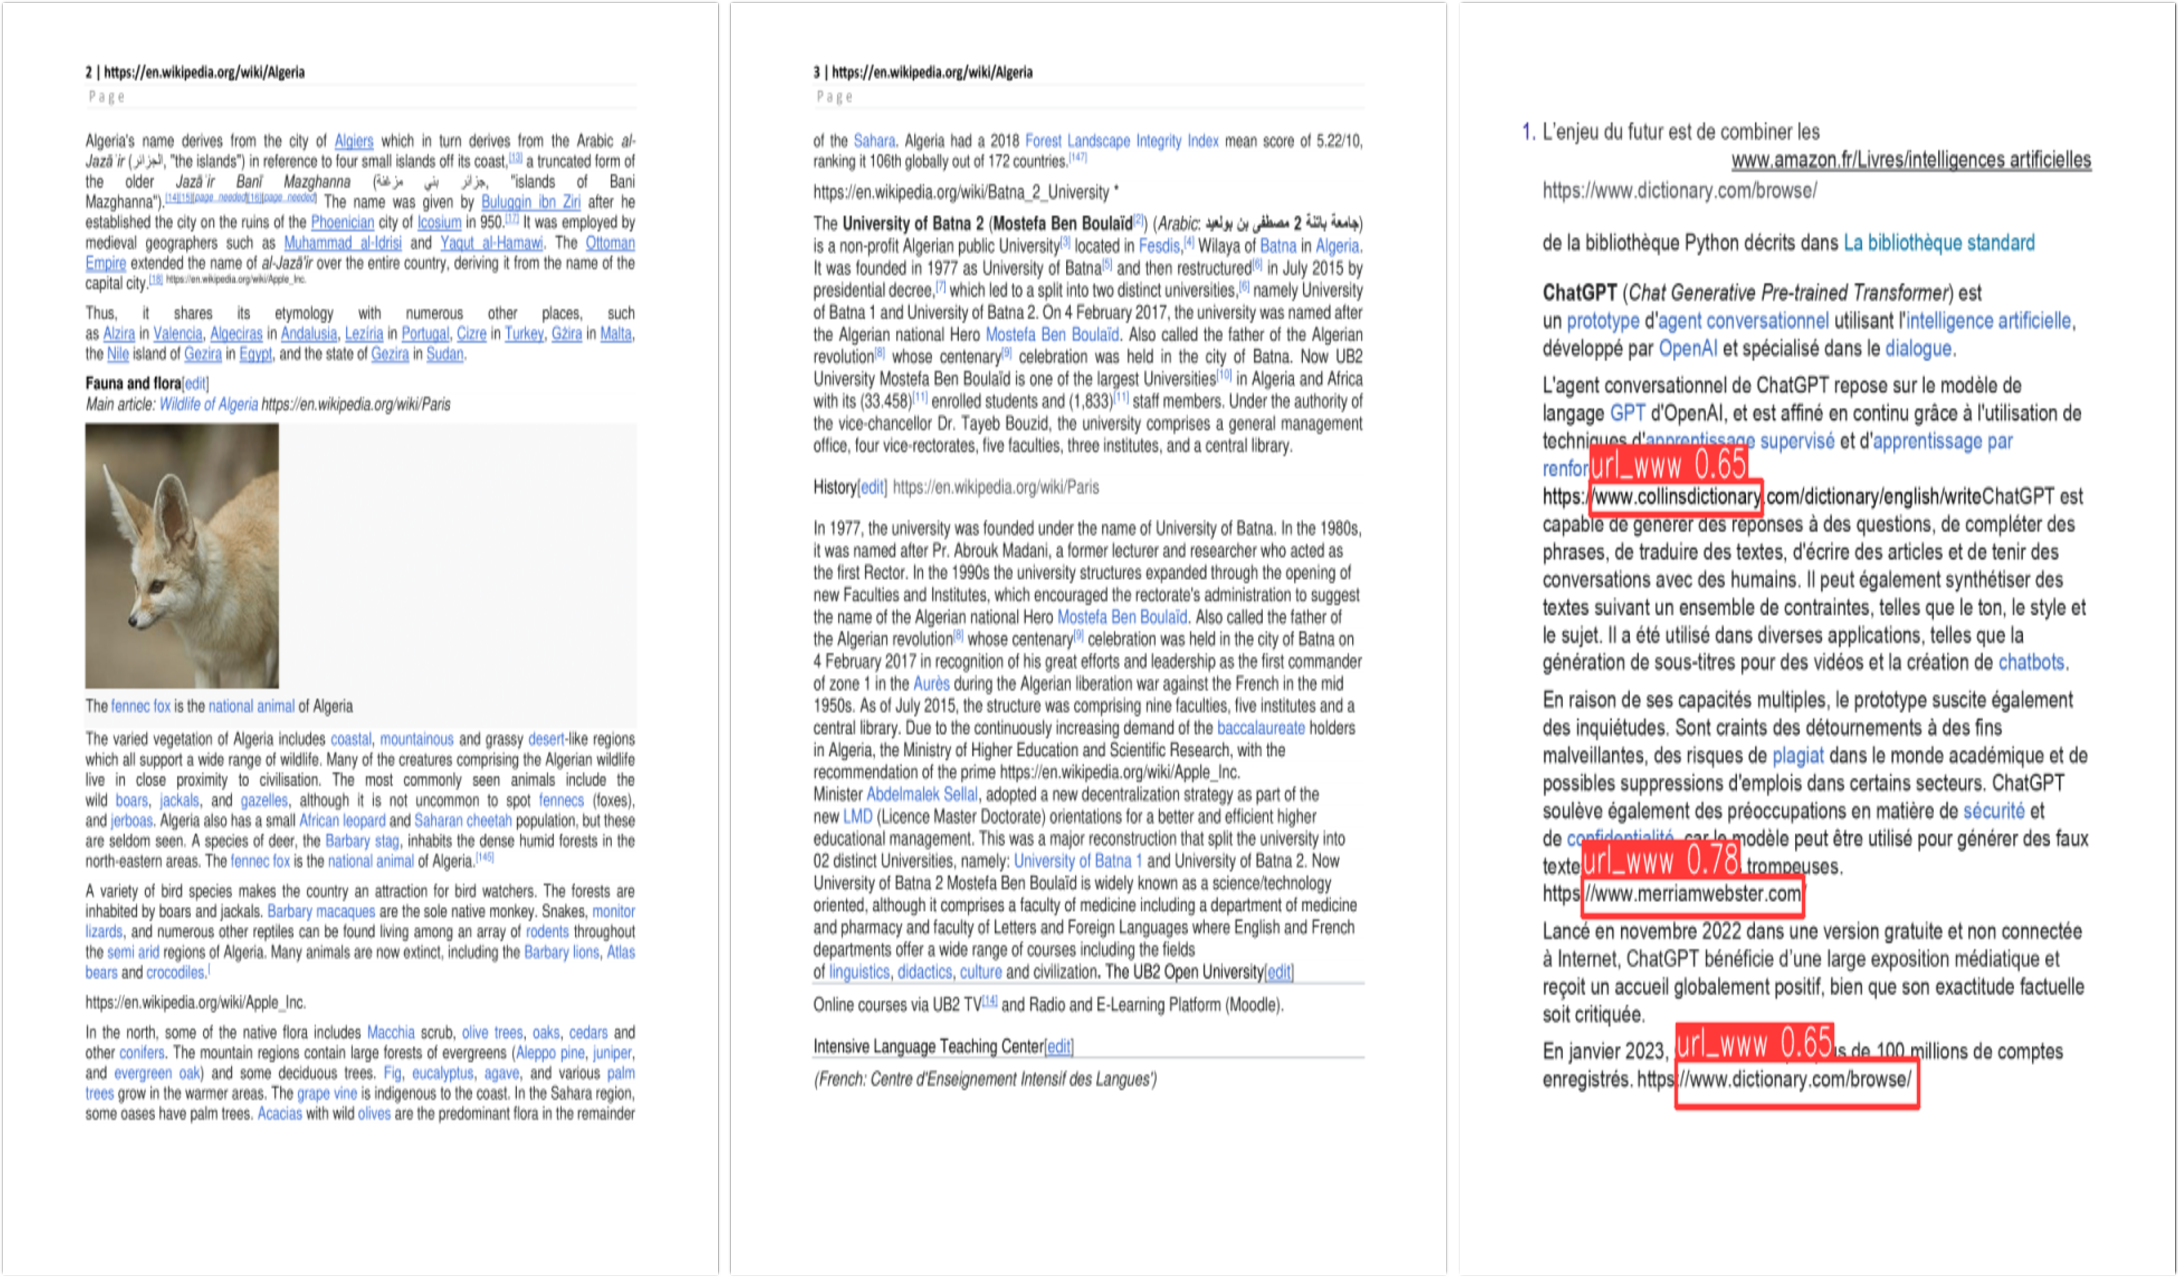
\includegraphics[height=9cm,width=17cm]{Chapitre3/https_yolov5.png}
                    \caption{Test de difficulté: URL préfixées avec la balise de protocole \textit{https://} - YOLOv5.}
                    \label{y5_https}
                    \end{figure}

          % ---------- MANUSCRIPT -----------
          \subsubsection{Caractères d'URL écrits en manuscrit}
          Tous les modèles ont échoué dans cette difficulté avec une précision moyenne de $0\%$.
          \begin{figure}[H]
                    \centering
                    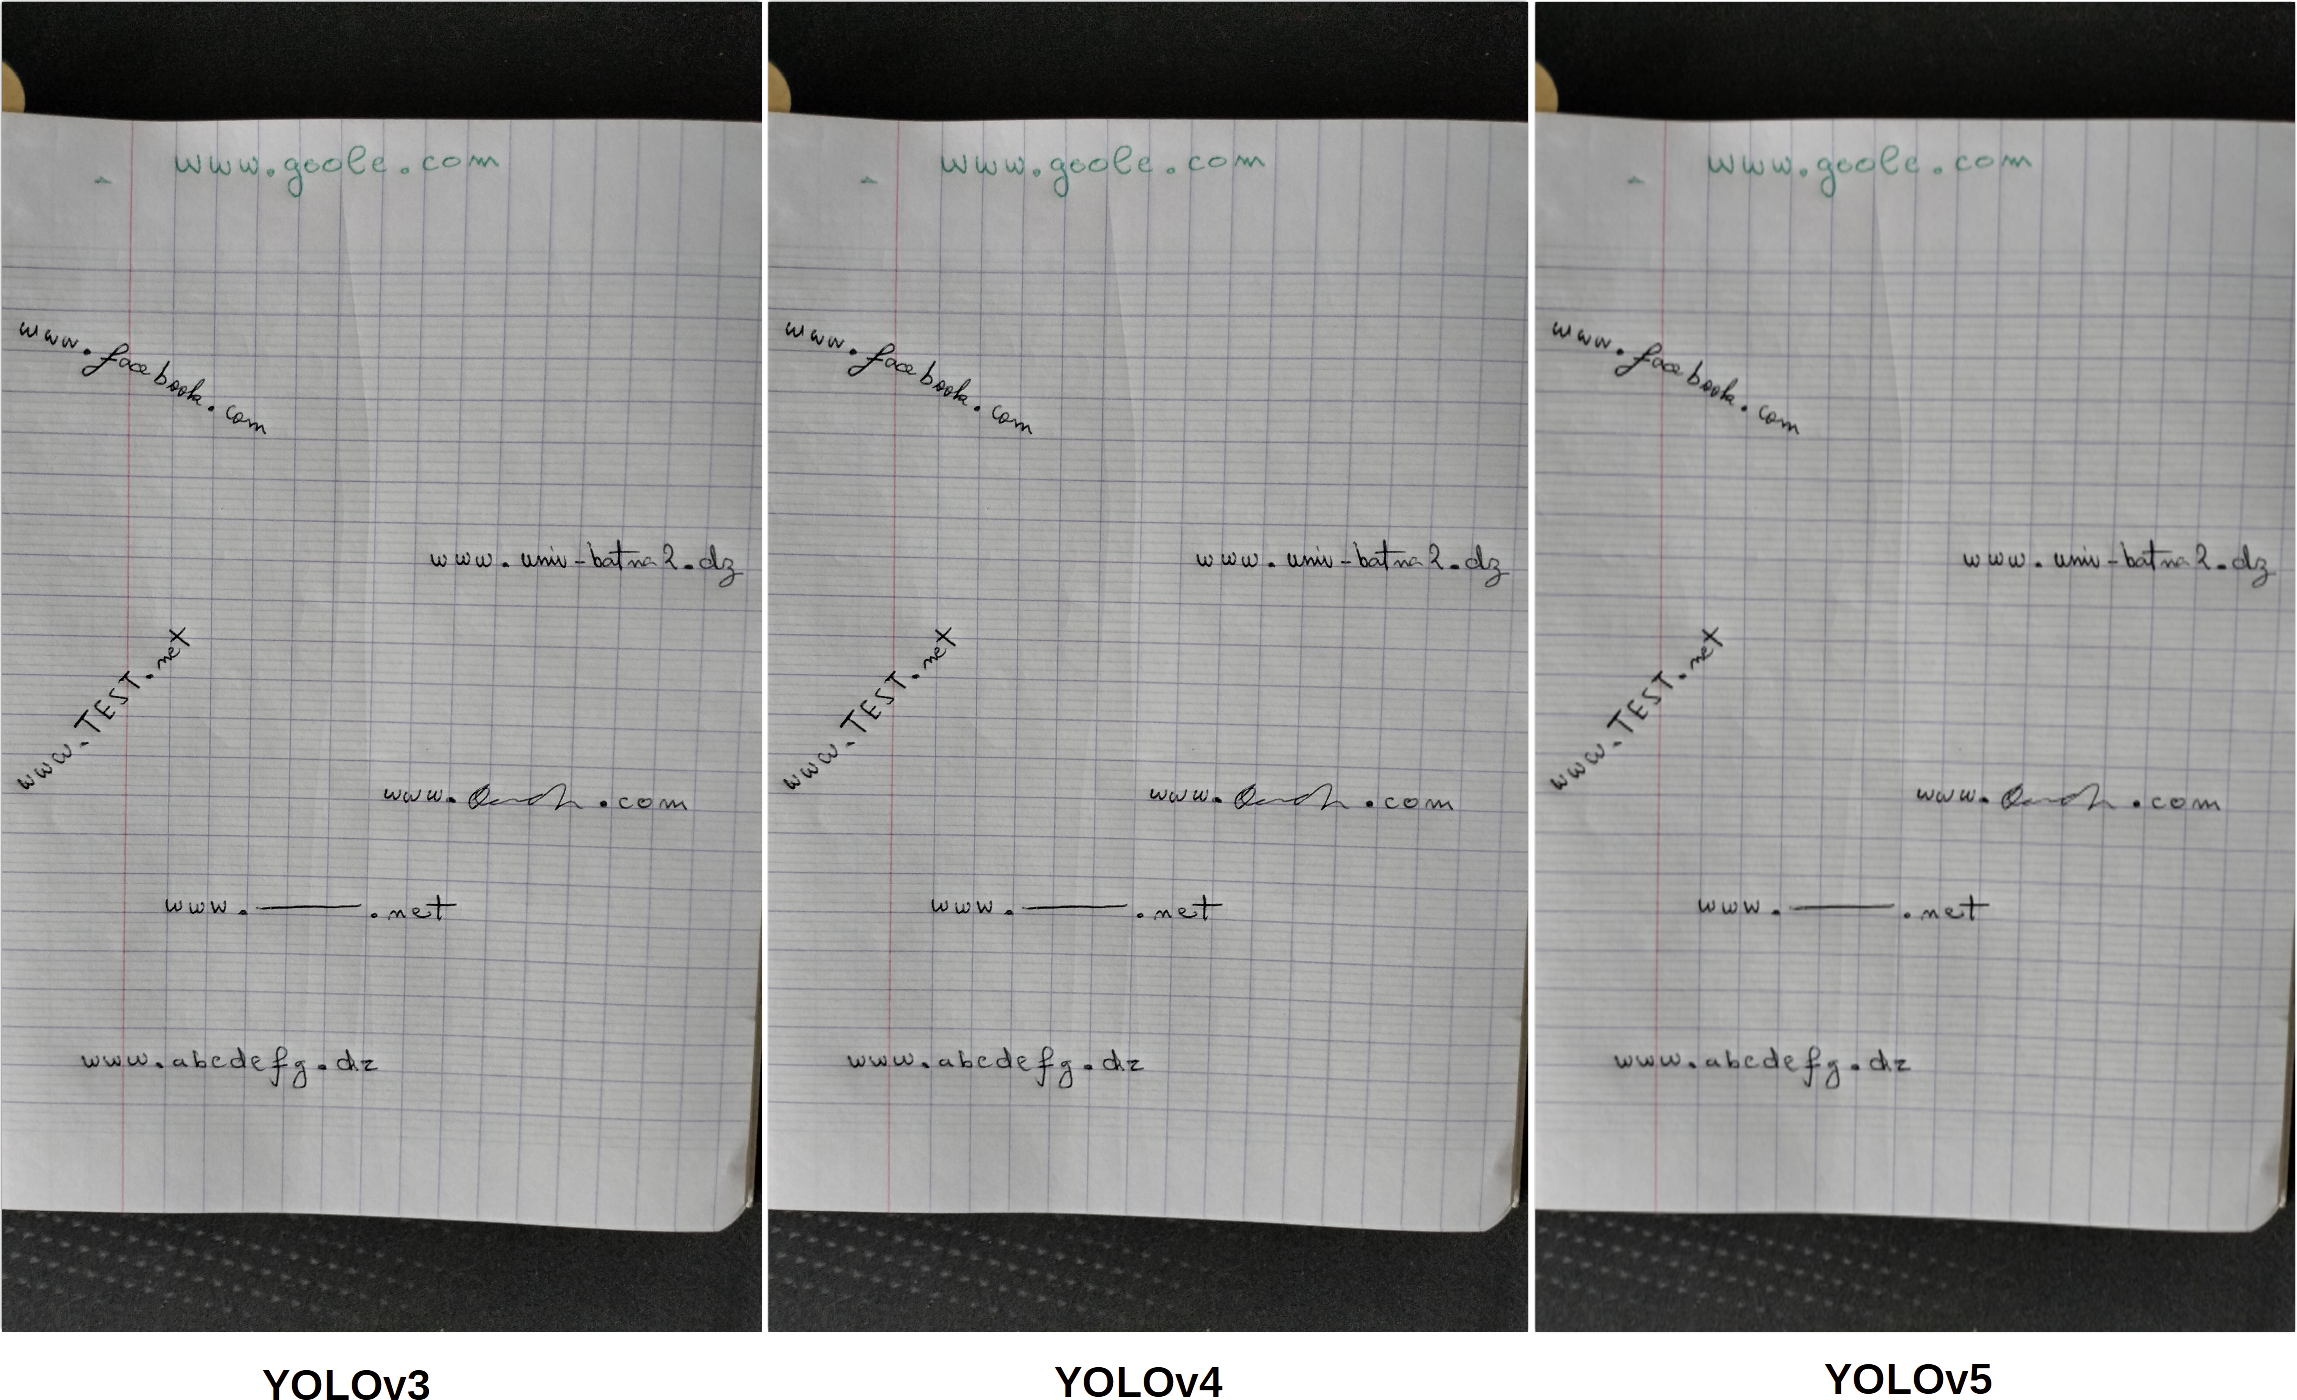
\includegraphics[height=7cm,width=17cm]{Chapitre3/test_manuscript.png}
                    \caption{Test de difficulté: Images avec Flou-GaussianCaractères d'URL écrits en manuscrit - YOLOv3 / YOLOv4 / YOLOv5.}
                    \label{test_manuscrit}
                    \end{figure}

          % ---------- FLOU ------------
          \subsubsection{Images avec Flou-Gaussian.}
          Le flou n'affecte pas beaucoup les performances des modèles. YOLOv3 a obtenu une précision moyenne de $72,73\%$. YOLOv4 a obtenu un score parfait de $100\%$ et YOLOv5 un score de $90,91\%$.
          \begin{figure}[H]
                    \centering
                    \includegraphics[height=9cm,width=17cm]{Chapitre3/blur_yolov3.png}
                    \caption{Test de difficulté: Images avec Flou-Gaussian - YOLOv3.}
                    \label{y3_blur}
                    \end{figure}
          \begin{figure}[H]
                    \centering
                    \includegraphics[height=9cm,width=17cm]{Chapitre3/blur_yolov4.png}
                    \caption{Test de difficulté: Images avec Flou-Gaussian - YOLOv4.}
                    \label{y4_blur}
                    \end{figure}
          \begin{figure}[H]
                    \centering
                    \includegraphics[height=9cm,width=17cm]{Chapitre3/blur_yolov5.png}
                    \caption{Test de difficulté: Images avec Flou-Gaussian - YOLOv5.}
                    \label{y5_blur}
                    \end{figure}

          % ---------- FLOU ------------
          \subsubsection{Images avec Bruit-Gaussian.}
          Contrairement au flou, le bruit affecte grandement la précision des modèles, il amène les modèles à détecter de faux objets.
          La précision YOLOv3 a chuté à $36,36\%$ et YOLOv4 a également chuté au même score de $36,36\%$. Contrairement aux deux, YOLOv5 a obtenu un score plus élevé de $83,98\%$.
          \begin{figure}[H]
                    \centering
                    \includegraphics[height=9cm,width=17cm]{Chapitre3/bruit_yolov3.png}
                    \caption{Test de difficulté: Images avec Bruit-Gaussian - YOLOv3.}
                    \label{bruit_y3}
                    \end{figure}
          \begin{figure}[H]
                    \centering
                    \includegraphics[height=9cm,width=17cm]{Chapitre3/bruit_yolov4.png}
                    \caption{Test de difficulté: Images avec Bruit-Gaussian - YOLOv4.}
                    \label{bruit_y4}
                    \end{figure}
          \begin{figure}[H]
                    \centering
                    \includegraphics[height=9cm,width=17cm]{Chapitre3/bruit_yolov5.png}
                    \caption{Test de difficulté: Images avec Bruit-Gaussian - YOLOv5.}
                    \label{bruit_y5}
                    \end{figure}
\section{Conlusion}
Dans cette section. nous avons mentionné la structure de l'objet que nous essayons de détecter et comment nous avons créé le jeu de données. Après cela. nous avons formé les 3 modèles avec $80\%$ de l'ensemble de données. Ensuite, nous avons évalué les modèles avec $20\%$ et nous les avons également évalués avec des difficultés connues.
D'après les évaluations, nous avons conclu que YOLOv4 est le plus robuste que YOLOv3 et YOLOv5.
